\documentclass{beamer}
\usepackage[utf8]{inputenc}
\usepackage{pifont}
\usetheme{Madrid}
\usecolortheme{default}

\documentclass{beamer}
\usepackage[utf8]{inputenc}
\usepackage{pifont}
\usepackage{caption}
\usetheme{Madrid}
\usecolortheme{default}

\usepackage{algorithm}
\usepackage{algorithmicx}
\usepackage{algpseudocode}
\usepackage{float}
\usepackage{tabularray}
\usepackage{xcolor} % Already included by tabularray
\UseTblrLibrary{booktabs}
\usepackage{booktabs}
\usepackage{tabularx}
%------------------------------------------------------------
%This block of code defines the information to appear in the
%Title page
\title[Power Analysis Side-channel Attacks] %optional
{Power Analysis Side-channel Attacks}

\subtitle{}

\author[Federico Zanca] % (optional)    
{Federico Zanca}

\institute[] % (optional)
{
  %\inst{1}%
  Computer Science and Engineering\\
  Politecnico di Milano
  %\and
  %\inst{2}%
  %Faculty of Chemistry\\
  %Very Famous University
}

\date[2025] % (optional)
{}

%\logo{\includegraphics[height=1cm]{overleaf-logo}}

%End of title page configuration block
%------------------------------------------------------------



%------------------------------------------------------------
%The next block of commands puts the table of contents at the 
%beginning of each section and highlights the current section:

\AtBeginSection[]
{
  \begin{frame}
    \frametitle{Table of Contents}
    \tableofcontents[currentsection]
  \end{frame}
}
%------------------------------------------------------------


\begin{document}

%The next statement creates the title page.
\frame{\titlepage}


%---------------------------------------------------------
%This block of code is for the table of contents after
%the title page
\begin{frame}
\frametitle{Table of Contents}
\tableofcontents
\end{frame}
%---------------------------------------------------------




\section{Introduction to Side-Channel Attacks}

\begin{frame}
    \frametitle{What Are Side-Channel Attacks?}

    \begin{block}{Definition}
        Side-channel attacks exploit unintended \textbf{physical leakages} from cryptographic devices to extract secret information.
        \begin{itemize}
            \item Instead of attacking the mathematical foundations of a cryptographic algorithm, they target information leaked through physical phenomena.
            \item This happens if there is a relationship between data/operations and a certain physical phenomena that can be observed
            \item Common leakage sources include \textbf{power consumption}, electromagnetic emissions, timing variations, and even sound or heat.
        \end{itemize}
    \end{block} 
\end{frame}

\begin{frame}{Why Are They Important?}
    \begin{block}{}
\textbf{A strong encryption algorithm is not secure if the underlying implementation is flawed
}        \begin{itemize}
            \item Many devices thought to be secure can be compromised by analyzing side-channels.
            \item Attackers can retrieve secret keys without breaking the cryptographic math.
            \item Real-world cryptographic implementations often leak enough information to be vulnerable.
        \end{itemize}
    \end{block}
    
First publicized power analysis attacks appeared in the late 1990s. \newline
Since then, the field has evolved to include a variety of sophisticated techniques and powerful countermeasures.
\end{frame}

\section{Power analysis}

% Slide 1: What is a Power Analysis Attack?
\begin{frame}
    \frametitle{What is a Power Analysis Attack?}

    \begin{alertblock}{}
        Switching 1 $\rightarrow$ 0 and 0 $\rightarrow$ 1 means providing or removing power to transistors.\newline
        A power analysis attack is a technique that exploits the relationship between a device's \textbf{power consumption} and the \textbf{data it processes}  or the \textbf{operations} performed.

        By carefully measuring power usage, an attacker can learn about the secret data being used
    \end{alertblock}

    
\end{frame}

\begin{frame}
    \frametitle{The Attack Setup}

        The setup for a power analysis attack is composed of:
        \begin{itemize}
            \item A \textbf{target device} that performs cryptography.
            \item A small \textbf{resistor} placed in the power line of the device.
            \item A digital \textbf{oscilloscope} to measure the tiny voltage changes across the resistor.
        \end{itemize}
        The oscilloscope captures a \textbf{power trace}: a graph of power usage over time.


    \begin{figure}
        \centering
        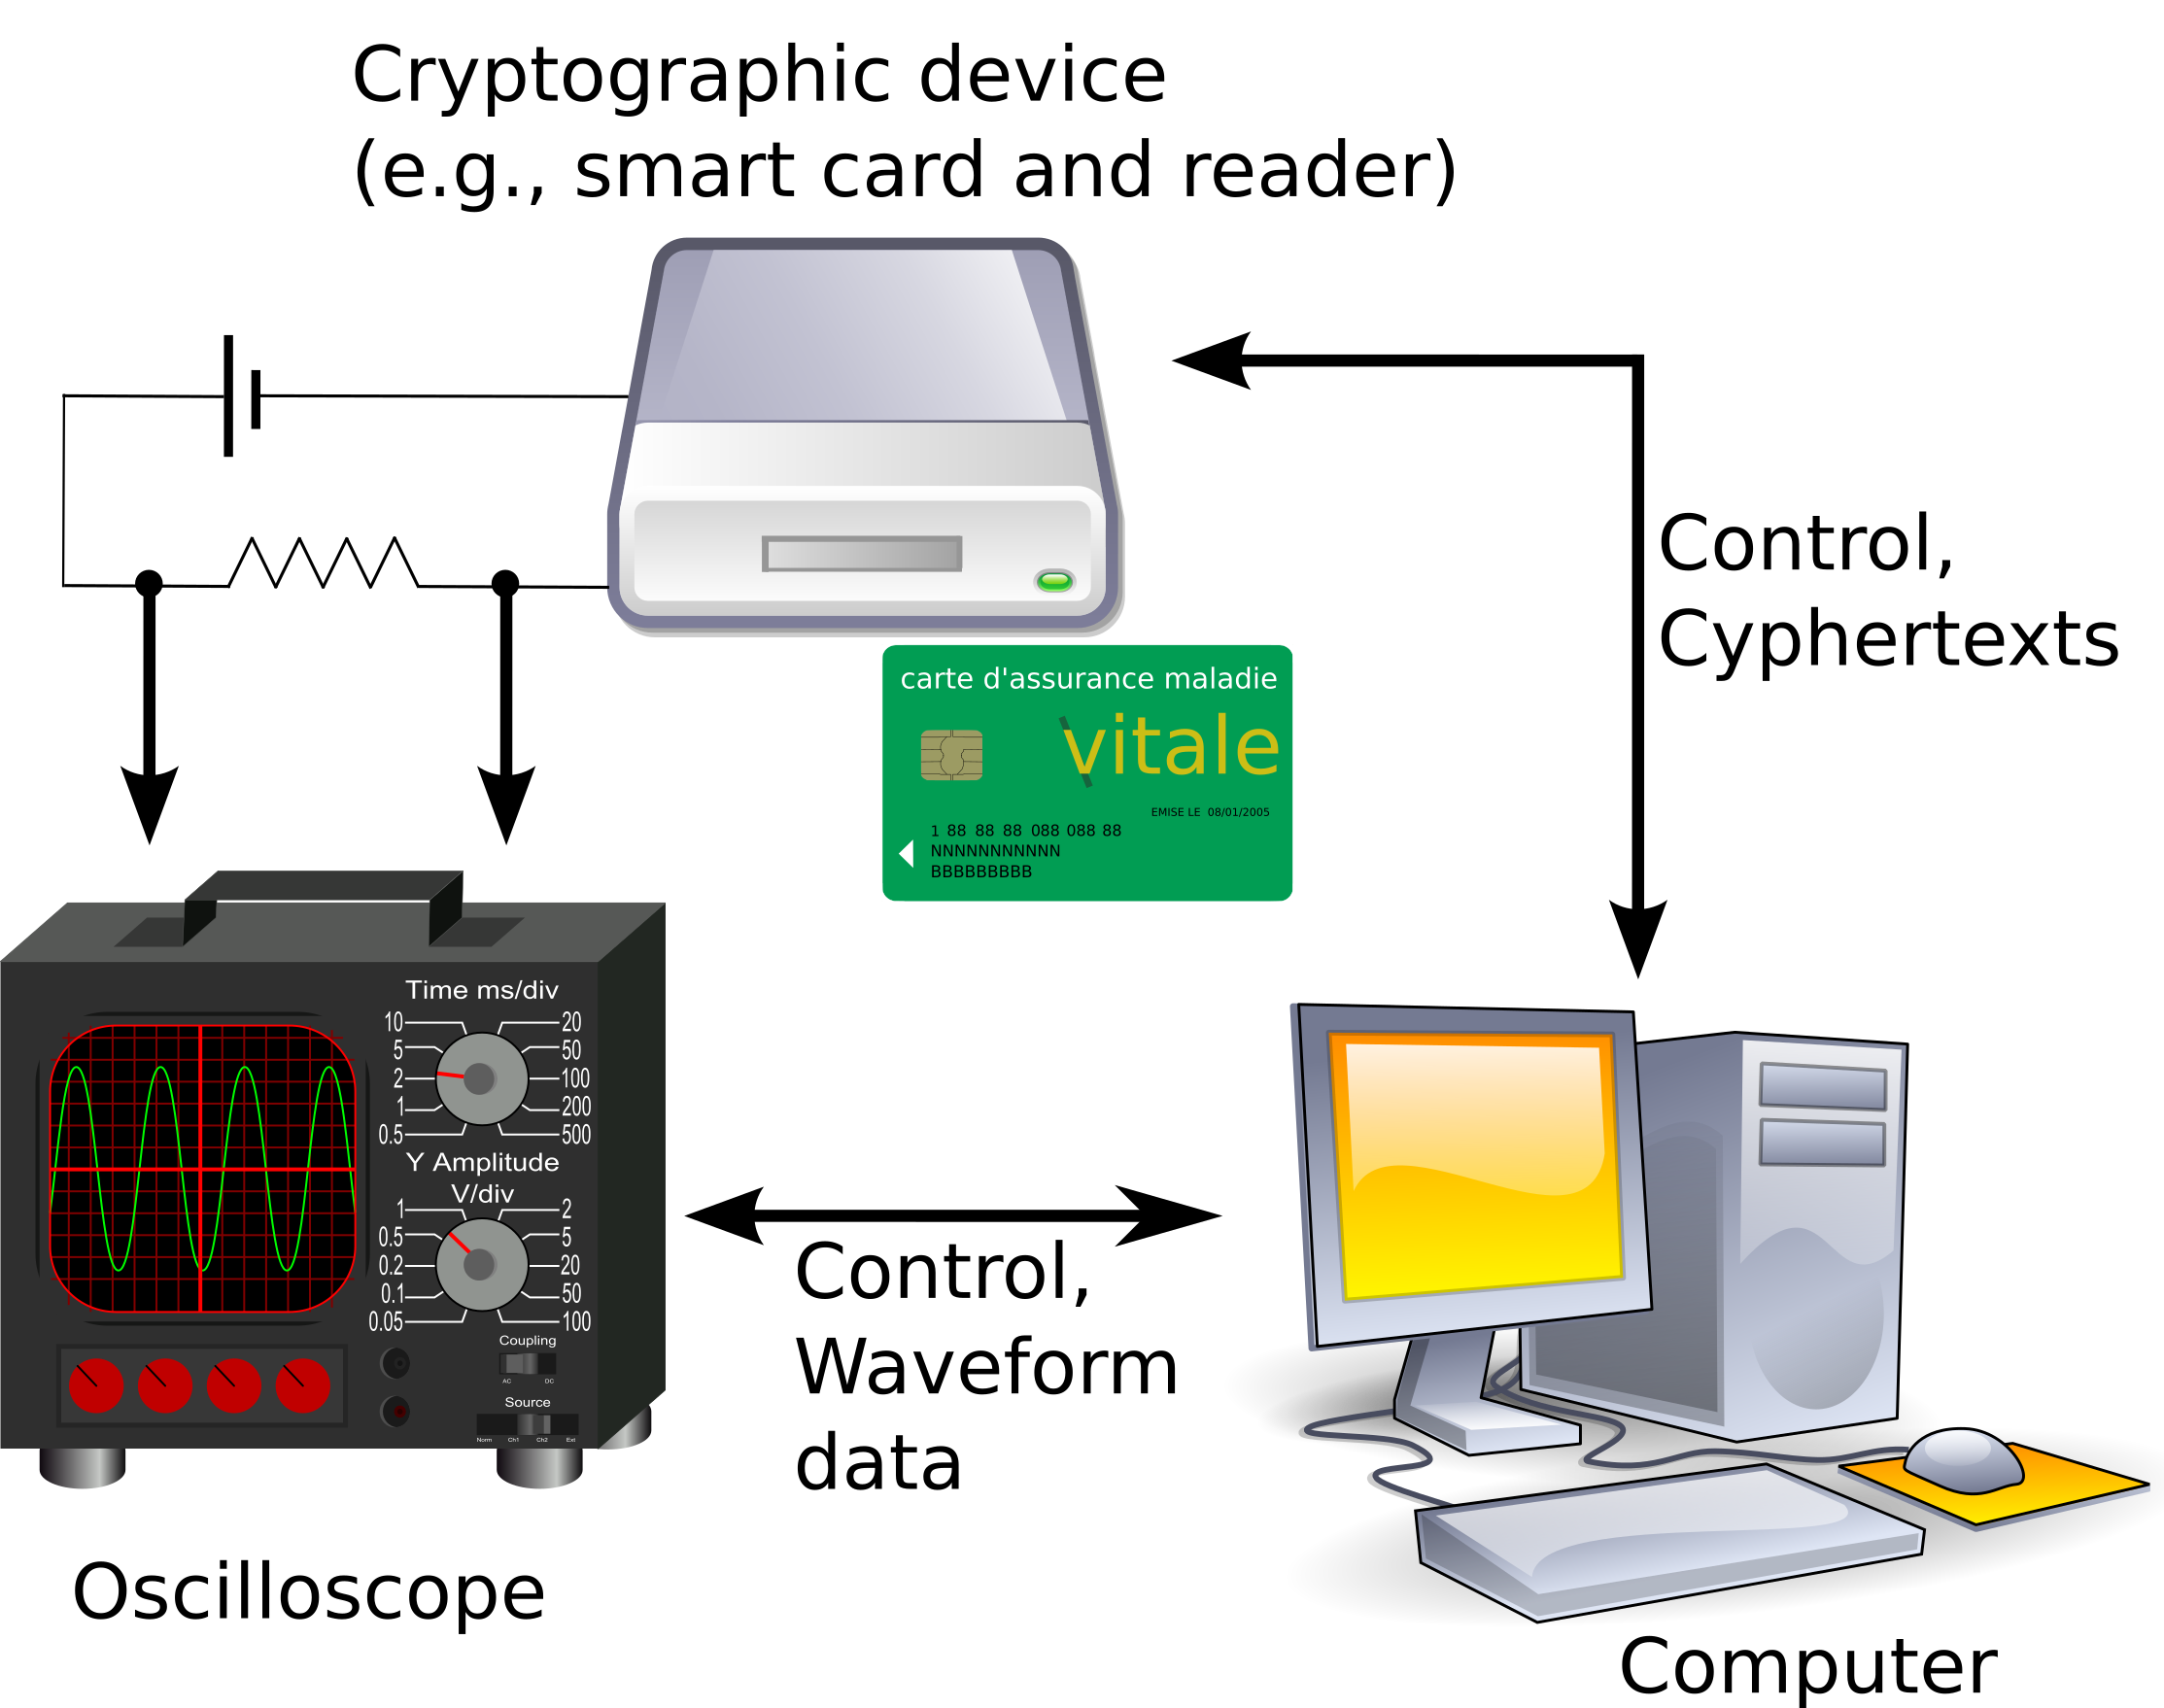
\includegraphics[width=0.45\textwidth]{main thing/Pictures/scheme2_oscilloscope.png}
       
    \end{figure}
\end{frame}

\begin{frame}
    \frametitle{Possible target devices}

    Electronic devices that perform cryptographic computations can be power analysis targets. This includes:
    \begin{itemize}
        \item Smart Cards and Security Tokens
        \item Embedded Microcontrollers (MCUs)
        \item Internet of Things (IoT) Devices
        \item Mobile Phones and Tablets
    \end{itemize}
    \begin{columns}[T] % The 'T' option aligns the columns at the top
        \begin{column}{0.40\textwidth}
            \centering
            
\includegraphics[width=\linewidth]{main thing/Pictures/smartcard.png}
        \end{column}
        
        \begin{column}{0.48\textwidth}
            \centering
            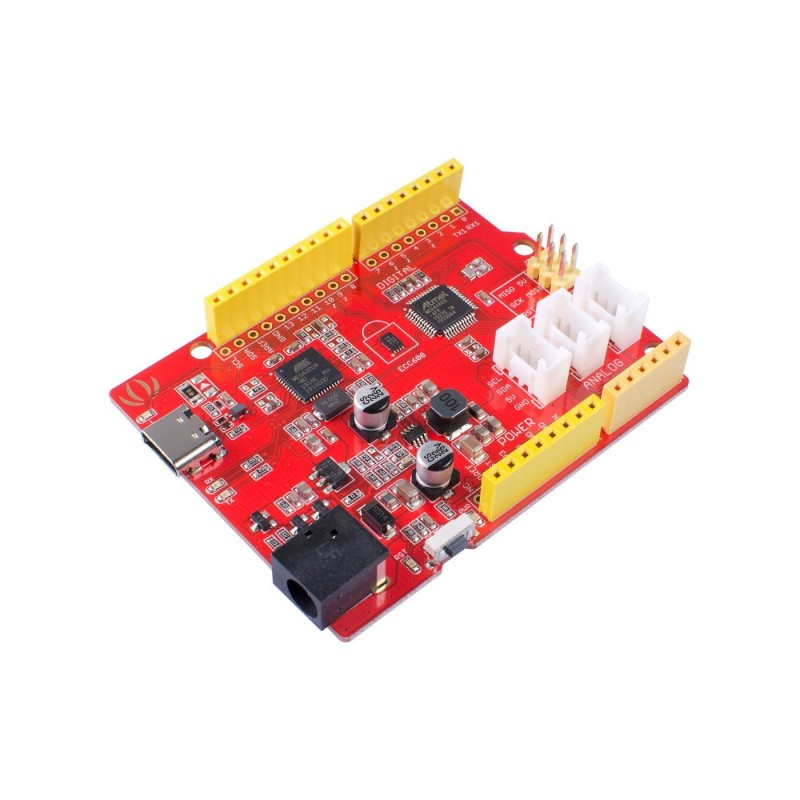
\includegraphics[width=\linewidth]{main thing/Pictures/mcu.jpg}
        \end{column}
    \end{columns}
\end{frame}

\begin{frame}
    \frametitle{The Goal of Power Analysis attacks}

    \begin{block}{Retrieving the Secret Key}
        The primary goal of most power analysis attacks is to recover secret \textbf{cryptographic keys}.
    \newline
        This is rarely done by attacking the full key at once. Instead, attackers target \textbf{intermediate values} that are processed during the cryptographic algorithm. By learning small pieces of the key one at a time, they can eventually reconstruct the entire secret.
    \end{block}
   
\end{frame}





\begin{frame}
    \frametitle{The Power Trace: A Measurement Vector}

    \begin{block}{Definition}
        A power trace is a discrete time-series vector representing the instantaneous power consumption of a cryptographic device during a specific operation.
        \begin{itemize}
            \item Each point in the trace corresponds to a power measurement at a discrete point in time, captured by a high-frequency sampling instrument like a digital oscilloscope.
            \item The trace represents the electrical activity of the device's components.
        \end{itemize}
    \end{block}

    \begin{figure}
        \centering
        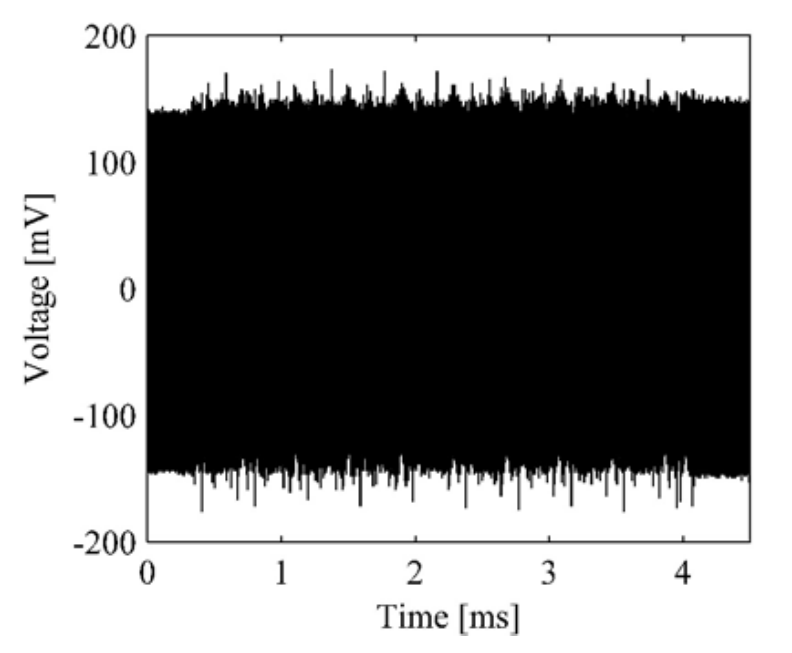
\includegraphics[width=0.35\linewidth]{main thing/Pictures/trace.png}
    \end{figure}
\end{frame}

\begin{frame}
    \frametitle{The Non-Deterministic Nature of Measurements}

    \begin{block}{The Problem of Measurement Variance}
        Repeated measurements of the same operation, using the \textbf{exact same inputs} (key and plaintext), will yield different power traces.\newline
        This variability is due to the presence of \textbf{noise}.
    \end{block}
    
    \begin{figure}
        \centering
        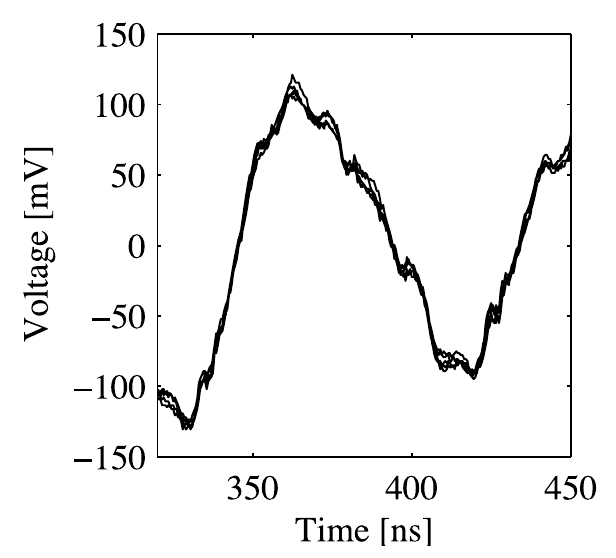
\includegraphics[width=0.4\linewidth]{main thing/Pictures/noise.png}
        \caption{Power traces are different (but look very similar) even processing the same input because of noise}
    \end{figure}
\end{frame}


\begin{frame}
    \frametitle{Noise Source 1: Electronic Noise}

    \begin{block}{The Stochastic Component}
        \textbf{Electronic Noise}, $P_{electronic\_noise}$, is originated by the physical properties of the electronic components and the measurement setup.\newline
        It has many sources:
        
        \begin{itemize}
            \item Power supply
            \item Clock generator
            \item Radiated emissions of neighboring components
        \end{itemize}
    \end{block}
    \begin{alertblock}{}
        The distribution of the electronic noise $P_{el.noise}$ is a normal distribution
        $$P_{el.noise} \sim \mathcal{N(0, \sigma)}$$
    \end{alertblock}
\end{frame}

\begin{frame}
    \frametitle{Noise Source 2: Switching Noise}

    \begin{block}{The Uncorrelated Component}
        \textbf{Switching Noise} is the variations of power traces that are caused by cells that are not relevant for the attack. 
        
        \begin{itemize}
            \item The amount of switching noise also depends on the architecture of the attacked device
            \item More computations performed in parallel by device $\rightarrow$ More switching noise
            \item The two most relevant properties of the measurement setup that introduce switching noise are the \textbf{clock frequency }of the device and \textbf{bandwidth} of the connection between the target logic cells and the oscilloscope
        \end{itemize}
    \end{block}
\end{frame}

\begin{frame}
    \frametitle{Composition of Power Traces}

    \begin{block}{Model of each point of a power trace}
        Each point of a power trace can be modeled as the sum of an operation-dependent component $P_{op}$, a data-dependent component $P_{data}$, electronic noise $P_{el.noise}$, and a constant component $P_{const}$.
        \vspace{0.5cm}
        $$ P_{total} = P_{op} + P_{data} + P_{el. noise} + P_{const} $$
        
        All of these components are a function of time; we do not write them explicitly that way as we usually only analyze single points based on this model.\newline
        $P_{const}$ is not relevant for power analysis attacks because it does not provide any exploitable information for an attacker.
    \end{block}
    \begin{alertblock}{}
        The distributions of $P_{op}$, $P_{data}$ and $P_{el.noise}$ can usually be approximated by a \textbf{normal distribution}.
    \end{alertblock}
\end{frame}

\begin{frame}
    \frametitle{Signal and Noise}

        In the context of a given attack scenario, the power consumption of a point of a power trace can be modeled as the sum of the exploitable power consumption $P_{exp}$, the switching noise $P_{sw.noise}$, the electronic noise $P_{el.noise}$ and the constant cmoponent $P_{const}$.

        
        \vspace{0.5cm}
        $$P_{total}=P_{exp}+P_{sw.noise}+P_{el.noise}+P_{const}$$
        \vspace{0.5cm}

        These components are independent of each other. Therefore, all parts of the power consumption that depend on the information that the attacker is looking for need to be modeled as $P_{exp}$ and not as $P_{sw.noise}$. 
\end{frame}


\begin{frame}
    \frametitle{Signal-to-Noise Ratio (SNR)}

        \textit{Signal-to-noise ratio} is the ratio between the signal and the noise component of a measurement $$SNR=\frac{Var(Signal)}{Var(Noise)}$$
    \begin{block}{Definition}
        In the context of a given attack scenario, the signal-to-noise ratio of a point of a power trace is given by the following equation
        
        \vspace{0.5cm}
        $$ \text{SNR} = \frac{\text{Var}(P_{exp})}{\text{Var}(P_{sw.noise}+P_{el.noise})} $$
        \vspace{0.5cm}
        
        The SNR quantifies how much information is leaking from a point of a power trace. The higher the SNR, the higher is the leakage
    \end{block}
\end{frame}

\begin{frame}
    \frametitle{The Role of SNR in Attack Efficiency}

    \begin{block}{SNR as an Indicator of Attack Feasibility}
        The SNR is a primary determinant of the efficiency and success of a power analysis attack.
        
        \begin{itemize}
            \item \textbf{High SNR}: Indicates that the data-dependent signal is strong relative to the noise. This allows for a successful attack with a smaller number of power traces.
            \item \textbf{Low SNR}: Indicates that the signal is weak and obscured by noise. A much larger number of traces is required to average out the noise and isolate the leakage.
        \end{itemize}
    \end{block}
    
        The number of traces ($N$) required for a successful attack is inversely proportional to the SNR:
        $$ N \propto \frac{1}{\text{SNR}} $$
        An attacker wants to maximize the SNR of their measurement setup, defender aims to design systems with the lowest possible SNR.
\end{frame}

\section{Simple Power Analysis (SPA)}

\begin{frame}
    \frametitle{Simple Power Analysis (SPA)}
    \begin{block}{What is SPA? }
        \begin{itemize}
            \item Attack technique based on the \textbf{direct visual interpretation} of power consumption traces from a cryptographic device.
            \item SPA attacks exploit key-dependent patterns within a trace
            \item They use only one trace (or very few traces)
            \item This was one of the first power analysis techniques to be publicly described.
        \end{itemize}
    \end{block}
\end{frame}

\begin{frame}
    \begin{figure}
        \centering
        \begin{minipage}{0.48\textwidth}
            \centering
            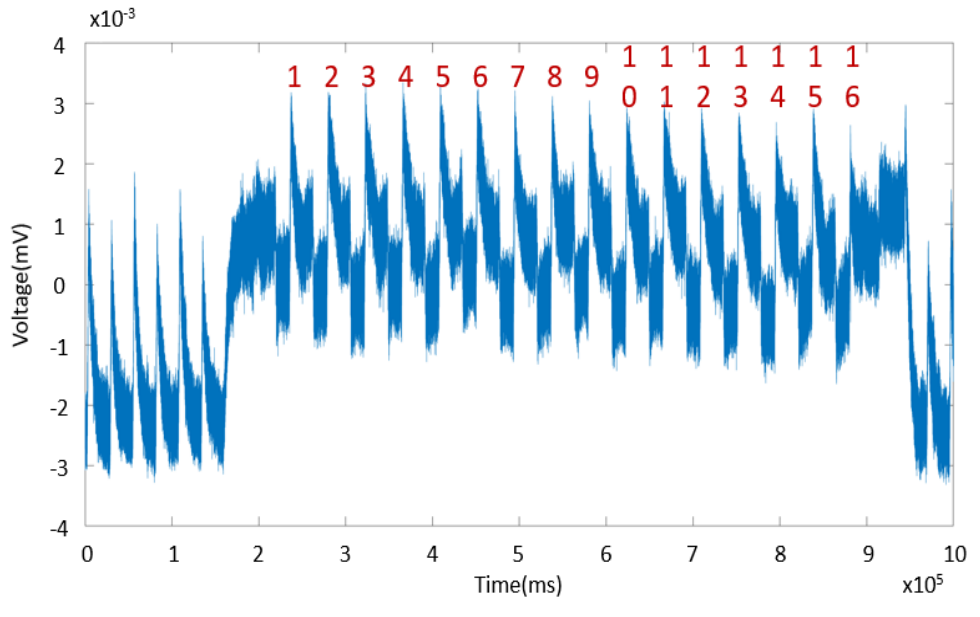
\includegraphics[width=\linewidth]{main thing/Pictures/DES_SPA_trace.png}
            \captionof{figure}{\small An SPA trace showing the 16 rounds of a DES encryption.}
        \end{minipage}\hfill
        \begin{minipage}{0.48\textwidth}
            \centering
            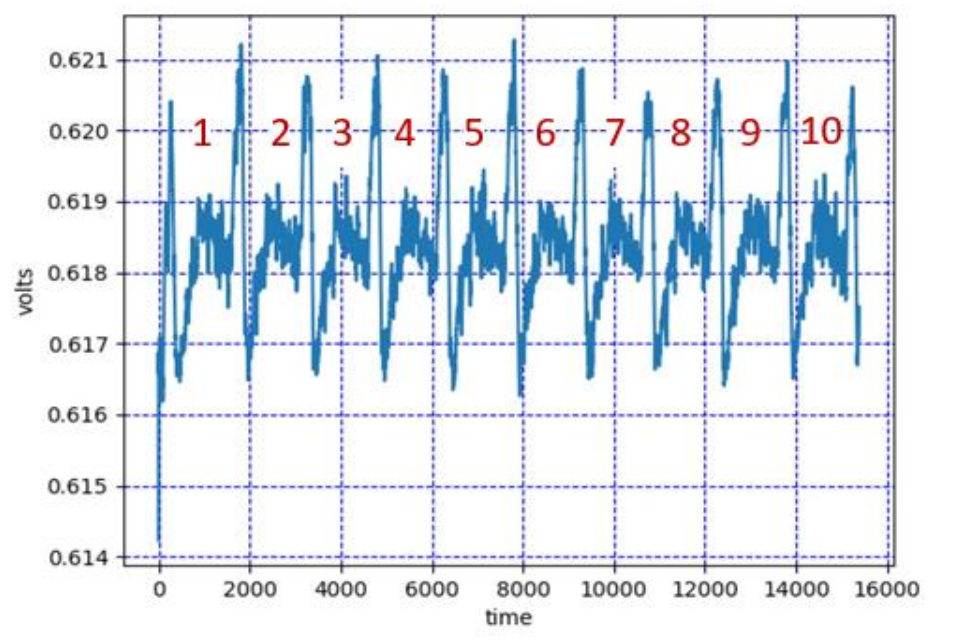
\includegraphics[width=\linewidth]{main thing/Pictures/AES_SPA_trace.png}
            \captionof{figure}{\small An SPA trace revealing the 10 rounds of an AES encryption.}
        \end{minipage}
    \end{figure}
\end{frame}


\begin{frame}
    \frametitle{Averaging Traces to Reduce Noise}

    The electrical signals measured are very small and inherently noisy. The random electronic noise component can obscure the underlying patterns.
    
    To improve the clarity of the trace for visual inspection, an attacker can capture multiple traces of the same operation and \textbf{compute their average}.
    
    \begin{alertblock}{}
         Since the electronic noise is typically \textbf{normally distributed} with a mean of zero, \textbf{averaging causes the noise to cancel out}. \newline
         The underlying deterministic signal, which is consistent across traces, is reinforced.
    \end{alertblock}
    
    This technique significantly improves the signal-to-noise ratio (SNR) for visual analysis.
\end{frame}

\begin{frame}
    \frametitle{Interpreting SPA Traces}

    By visually inspecting a power trace, an attacker can identify large-scale features of the cryptographic algorithm.
    
    \begin{itemize}
        \item \textbf{Algorithmic Rounds:} Iterative ciphers like DES and AES produce repetitive patterns, where each repetition corresponds to one round of the algorithm.
        \item \textbf{Distinct Operations:} Different operations within a round, such as substitutions (S-boxes) and permutations (MixColumns), can consume different amounts of power and time, making them distinguishable in the trace.
    \end{itemize}

    This allows an attacker to map the power trace to the known structure of the cryptographic algorithm.
\end{frame}

\begin{frame}
    \begin{figure}
        \centering
        \begin{minipage}{0.48\textwidth}
            \centering
            % Replace with the path to your detailed AES trace image
            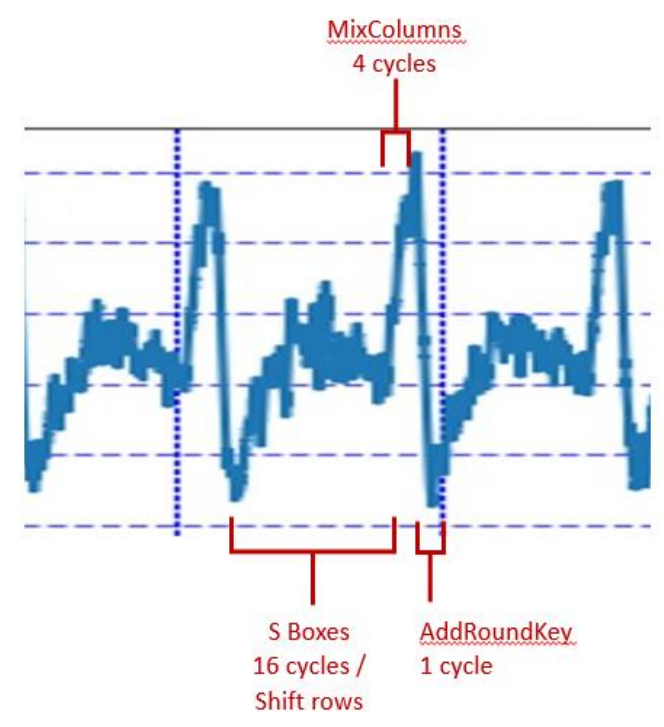
\includegraphics[width=\linewidth]{main thing/Pictures/detailed_AES_SPA_trace.png}
            \captionof{figure}{\small A detailed view of an AES round.}
        \end{minipage}\hfill
        \begin{minipage}{0.48\textwidth}
            \centering
            % Replace with the path to your AES block diagram image
            \includegraphics[width=\linewidth]{path/to/your/AES_diagram.png}
            \captionof{figure}{\small The standard block diagram of an AES round for comparison.}
        \end{minipage}
    \end{figure}
\end{frame}


\begin{frame}
    \frametitle{Classic SPA Attack: RSA Exponentiation}
    
    A classic example of SPA is the attack on RSA implementations that use the \textbf{square-and-multiply} algorithm for modular exponentiation.

    \begin{itemize}
        \item The algorithm processes the private key one bit at a time.
        \item If the key bit is a '1', it performs a \textbf{square} operation followed by a \textbf{multiply} operation.
        \item If the key bit is a '0', it performs \textbf{only a square} operation.
    \end{itemize}
    
    The additional 'multiply' operation for a '1' bit consumes a different amount of power and takes a different amount of time, creating a distinct and easily recognizable pattern in the power trace.
\end{frame}


\begin{frame}
    \frametitle{Visualizing the RSA Attack}
    
    By observing the sequence of power consumption patterns, an attacker can directly read the bits of the private exponent from the trace.

    \begin{figure}
        \centering
        % Replace with the path to your RSA trace image
        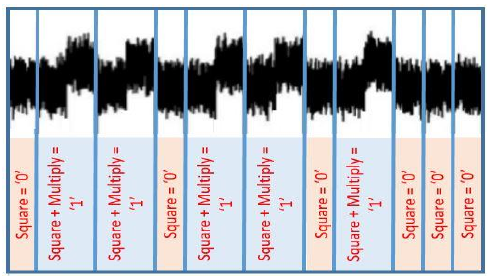
\includegraphics[width=0.8\linewidth]{main thing/Pictures/rsa_exponent.png}
        \captionof{figure}{\small A power trace of an RSA exponentiation. The distinct patterns for 'square' and 'square-and-multiply' operations reveal the secret key bits.}
    \end{figure}

  
\end{frame}
\section{Leakage Power Models}

\begin{frame}
    \frametitle{Two Classes of Power Analysis Attacks}

    Over time, power analysis attacks have divided into two main categories:

    \begin{itemize}
        \item \textbf{Model-Based Attacks:}
        \begin{itemize}
            \item Rely on assumed \textbf{power leakage models} to relate device power consumption to secret data.
            \item Use statistical techniques (difference of means, correlation, etc.) to test if a key guess matches observed traces.
            \item \textbf{Differential Power Analysis} and \textbf{Correlation Power Analysis} fall in this category
        \end{itemize}
        \item \textbf{Profiling Attacks:}
        \begin{itemize}
            \item Use a profiling device (a surrogate of the target) to empirically build a model of how the key affects leakage.
            \item Attack proceeds by matching new traces to the prebuilt “stencil” of leakages.
            \item \textbf{Template Attacks} fall in this category
        \end{itemize}
    \end{itemize}

    In both approaches, the effectiveness depends on how accurately the power model describes the real leakage behavior.
\end{frame}

\begin{frame}
    \frametitle{Power Models}

    \begin{block}{What is a Power Model?}
        A \textbf{power model} mathematically predicts how a device’s power consumption depends on the intermediate values manipulated by a cryptographic algorithm.
    \end{block}

    \vspace{0.5em}

    Power models are essential for model-based statistical attacks; they map the algorithm’s internal computations (e.g., AES S-box outputs) to hypotheses about power consumption, and allow attackers to use observed traces to distinguish key guesses.
\end{frame}

\begin{frame}
    \frametitle{Typical Power Models Used in SCA}

    Standard models include:

    \begin{itemize}
        \item \textbf{Hamming Weight (HW):} Number of “1” bits in a byte or word ($HW(x) = \sum_i x_i$) is related to power consumption
        \item \textbf{Hamming Distance (HD):} Number of bits that flip between two values ($HD(x, y) = HW(x \oplus y)$) is related to power consumption
        \item \textbf{Least Significant Byte (LSB):} Power consumption is related to the value of LSB
        \item \textbf{Zero Value (ZV):} Power spikes when intermediate value = 0 (due to gate level effects)
        \item \textbf{Multivariate/Learned Models}: Combines multiple leakage sources
    \end{itemize}
\end{frame}

\begin{frame}
    \frametitle{How Power Models Enable Statistical Attacks}

    \begin{itemize}
        \item Statistical attacks use the power model to \textbf{make hypotheses}: for each key guess, predict the hypothetical leakage at every trace.
        \item Measurements are grouped/binned by predicted value.
        \item Statistics (such as mean, correlation, or likelihood score) are computed for each hypothesis.
        \begin{block}
            \item The correct key is identified as the one whose hypothesis gives the highest statistical match to the observed physical traces.
        \end{block}
    \end{itemize}
\end{frame}

\section{Differential Power Analysis (DPA)}

\begin{frame}
    \frametitle{Differential Power Analysis }

    \textbf{Differential Power Analysis (DPA)} is a statistical method designed to identify data-dependent correlations in power measurements.

    The technique partitions sets of power traces into two subsets and computes the difference of the averages for those subsets.

    \begin{block}{Key Insight}
         If the subsets are \textbf{truly correlated} with secret-dependent power, their \textbf{average power traces will differ}.\newline If not, the difference between averages approaches zero as the number of traces increase.
    \end{block}

    This allows even very small correlations to be statistically isolated despite noise.
\end{frame}


\begin{frame}
    \frametitle{Detecting Leakage}

    By computing the difference between the average traces of the two subsets at each time point:

    \begin{itemize}
      \item Significant non-zero differences indicate a correlation with secret data.

      \item As the dataset grows, random noise averages out, revealing the leakage signal.

      \item This process can be automated across entire traces without prior knowledge of where leakage occurs.
    \end{itemize}
\end{frame}

\begin{frame}
    \frametitle{DPA: General Overview of the Algorithm}    
    \begin{enumerate}
        \item \textbf{Measure:} Capture a large number power traces with the victim device given a set of inputs.
        \item \textbf{Define a Selection Function:} A function that predicts a single bit of an intermediate value inside the cryptographic algorithm, based on a known value (like plaintext or ciphertext) and a \textit{guess} for a part of the key.
        
        \item \textbf{Partition Traces:} For a specific \textit{key guess}, classify all captured traces into two bins: one where the selection function predicts '0', and one where it predicts '1'.
        
        \item \textbf{Compare the Sets:} Calculate the average trace for each of the two sets. Then, compute the pointwise difference between these two average traces.
    \end{enumerate}
    \begin{block}{}
        \textbf{Key guess correct:} a "spike" will appear in the difference trace. \newline 
        \textbf{Key guess wrong:} partitioning is random, and the difference trace will be close to zero.
    \end{block}
\end{frame}


% Slide: Example: Visualizing DPA Averages and Differences
\begin{frame}
    \frametitle{Visualizing DPA Results: Case Study}

    

        \begin{itemize}
            \item The \textbf{top trace} is the average of all measured traces where the LSB was 1 (over the first two rounds of AES).
            \item The \textbf{second trace} is the average where the LSB was 0.
        \end{itemize}
        The two averages are visually very similar—differences due to leakage are much smaller than overall power consumption variations.

    % Place for figure inclusion
    \begin{figure}
        \centering
        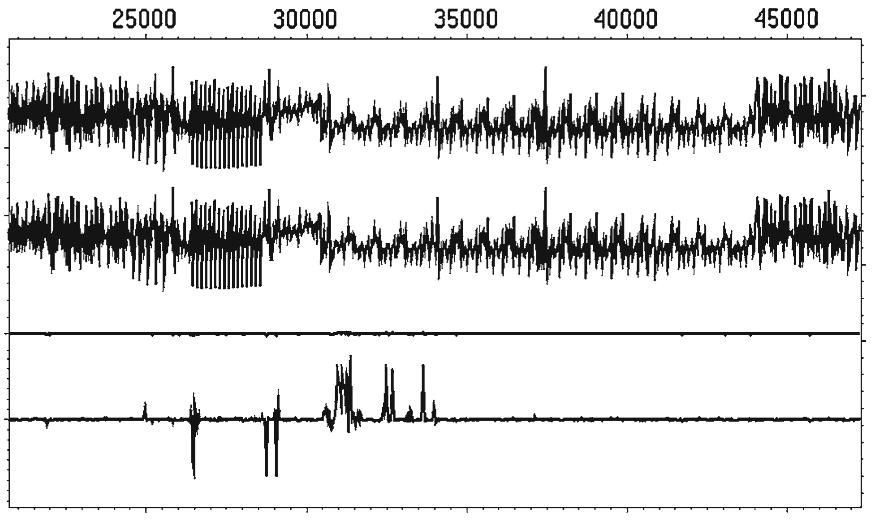
\includegraphics[width=0.60\textwidth]{main thing/Pictures/DPA_classic.png}
        \caption{Outcome of a DPA experiment against an AES smart card. The analysis targets the LSB of the first S-box output in the first round.}
    \end{figure}
\end{frame}


\begin{frame}
    \frametitle{Making Leakage Visible}

    \begin{itemize}
        \item The \textbf{third trace} in the figure shows the difference between the two subset averages. This line appears mostly flat, as the differences are small and masked by the y-axis scale.
        \item The \textbf{bottom trace} is the same difference but scaled up (e.g. $\times 15$), making the leakage spikes clearly visible.
    \end{itemize}

    \begin{block}{Leakage Interpretation}
        Spikes in the scaled difference trace correspond to moments when the targeted S-box output bit is manipulated inside the device. Spikes disappear after the first round, when the internal state is no longer correlated with the targeted bit.
    \end{block}

    High numbers of traces (e.g., 4,000) reduce noise, making the leakage clearer.
\end{frame}

% Slide: The Role of Selection Functions in DPA
\begin{frame}
    \frametitle{Selection Functions in Differential Power Analysis}

    The effectiveness of a DPA test critically depends on the choice of \textbf{selection function}.

    \begin{block}{Definition}
        A selection function is \textbf{used to assign traces to subsets} and is typically based on an educated guess as to a possible value for one or more intermediate values within a cryptographic calculation
    \end{block}
    Selection functions can be as simple as the predicted output bit of an S-box, or more complex, combining multiple bits or difference values.
    \begin{alertblock}{}
    \begin{itemize}
    \item If the final DPA trace shows \textbf{significant spikes}, the \textbf{selection function is correlated} with an internal value computed by the device.
        \item If not, the prediction is either \textbf{incorrect} or too weakly correlated to detect.
        \end{itemize}
    \end{alertblock}
\end{frame}


% Slide 1: DPA Targets the First Round of AES
\begin{frame}
    \frametitle{DPA Attack on AES-128: Overview}

    To illustrate the DPA process, we examine a classic attack on AES-128 encryption using real power traces from a smart card device. \newline
    \begin{block}{Quick memory refresher on AES}
        \begin{itemize}
            \item AES is a block cipher (symmetric)
            \item AES runs in multiple \textbf{rounds}; each round performs 4 operations
            \item AES takes blocks of 16 bytes as input and a key that is 16 (AES-128), 24 (AES-192) or 32 (AES-256) bytes long 
            \item Plaintext and ciphertext are always the same size
        \end{itemize}
    \end{block}
    We will attack the first round of AES.
\end{frame}

\begin{frame}{AES-128 Rounds}
     \begin{figure}
    
        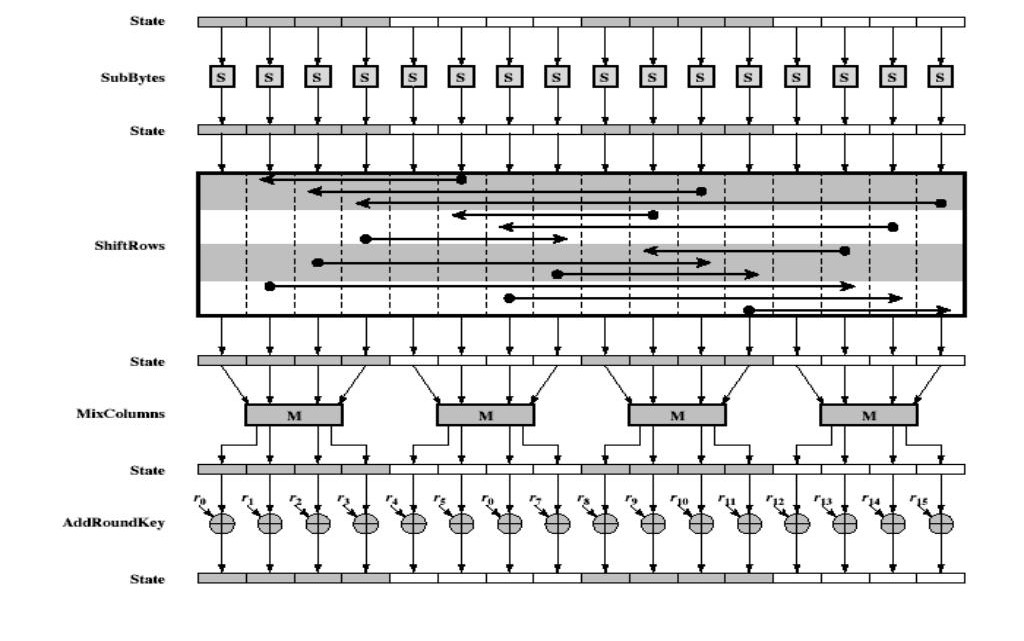
\includegraphics[width=1\textwidth]{main thing/Pictures/aes-round-l.jpg}
        
    \end{figure}
\end{frame}


\begin{frame}
    \frametitle{AES-128 Round 1: Steps and Target}

    The first round of AES-128 consists of these steps:
    \begin{enumerate}
        \item \textbf{Initialization:} State is set to the 16-byte plaintext.
        \item \textbf{AddRoundKey:} The 16-byte secret key is XORed with the state.
        \item \textbf{SubBytes:} Each state byte is substituted using the S-box.
        \item \textbf{ShiftRows:} Each row is cyclically shifted.
        \item \textbf{MixColumns:} Each column is mixed by a linear operation.
    \end{enumerate}

    \begin{figure}
        \centering
        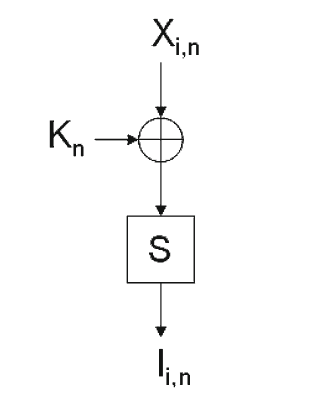
\includegraphics[width=0.25\textwidth]{main thing/Pictures/AddRoundKey_SBox_Diagram.png}
        \caption{The DPA attack focuses on the output of \textit{AddRoundKey} and \textit{SubBytes}, as shown in the figure.}
    \end{figure}
    
\end{frame}


\begin{frame}
    \frametitle{Intermediate Value \& Attack Notation}

    For each power trace $i$:
    \begin{itemize}
        \item $X_{i,n}$: The $n^{th}$ byte of plaintext in trace $i$ (known).
        \item $K_n$: The unknown $n^{th}$ byte of the round key (to be recovered).
        \item $I_{i,n}$: The $n^{th}$ byte of the state after SubBytes in round 1.
    \end{itemize}
    \begin{block}{}
    These terms are related:
    \[
        I_{i,n} = S[X_{i,n} \oplus K_n]
    \]
    where $S[\cdot]$ denotes the AES S-box.
    \end{block}
\end{frame}


\begin{frame}
    \frametitle{Key Search Strategy in DPA}

    Since $X_{i,n}$ is known, $K_n$ is unknown, and $S[\cdot]$ is public:

    \begin{itemize}
        \item For a candidate $K_n$, compute $I_{i,n}$ for each trace.
        \item Use a \textbf{selection function} (e.g., take the LSB of $I_{i,n}$) to assign each trace to subset 0 or 1.
        \item Repeat for all 256 possible values of $K_n$. Each round key requires only 256 guesses.
    \end{itemize}

\begin{block}{DPA Advantage}
        This divide-and-conquer method makes brute-force keyspace attack on AES feasible by turning a $2^{128}$ search into a succession of practical $2^8$ (256) searches. \newline
    DPA tests which candidate $K_n$ aligns with actual device leakage, byte by byte, to reveal the full 128-bit AES key.
    \end{block}
\end{frame}
% Slide 1: Subset 0
\begin{frame}
    \frametitle{Key Guess \textcolor{orange}{0x01} Binning Example}
    
    \centering
    \begin{tblr}{
        width = 0.8\linewidth,
        colspec = {Q[c,$]Q[c,$]Q[c,$]Q[c,$]Q[c,$]},
        row{1} = {cyan9, font=\bfseries},
        row{even} = {gray9},
        row{odd} = {white},
        hlines,
        vlines,
    }
        Input Data & Key Guess & XOR Output & S-Box Output & Subset \\
        \texttt{0xC7} & \texttt{0x01} & \texttt{0xC6} & \texttt{0xC7} & \textcolor{blue}{0} \\
        \texttt{0x1F} & \texttt{0x01} & \texttt{0x1E} & \texttt{0x1F} & \textcolor{blue}{0} \\
        \texttt{0x2C} & \texttt{0x01} & \texttt{0x2D} & \texttt{0x2C} & \textcolor{blue}{0} \\
        \texttt{0x89} & \texttt{0x01} & \texttt{0x88} & \texttt{0x89} & \textcolor{blue}{0} \\
        \texttt{0x01} & \texttt{0x01} & \texttt{0x00} & \texttt{0x01} & \textcolor{red}{\textbf{1}} \\
        \texttt{0xD2} & \texttt{0x01} & \texttt{0xD3} & \texttt{0xD2} & \textcolor{blue}{0} \\
    \end{tblr} \newline \newline
        \centering \textit{More traces are needed of course}
    
    
    
\end{frame}
% Slide 2: Subset 1
\begin{frame}
    \frametitle{Key Guess \textcolor{orange}{0x3D} Binning Example}
    
    \centering
    \begin{tblr}{
        width = 0.8\linewidth,
        colspec = {Q[c,$]Q[c,$]Q[c,$]Q[c,$]Q[c,$]},
        row{1} = {cyan9, font=\bfseries},
        row{even} = {gray9},
        row{odd} = {white},
        hlines,
        vlines,
    }
        Input Data & Key Guess & XOR Output & S-Box Output & Subset \\
        \texttt{0xC7} & \texttt{0x3D} & \texttt{0xFA} & \texttt{0x2D} & \textcolor{red}{1} \\
        \texttt{0x1F} & \texttt{0x3D} & \texttt{0x22} & \texttt{0x93} & \textcolor{red}{1} \\
        \texttt{0x2C} & \texttt{0x3D} & \texttt{0x11} & \texttt{0x82} & \textcolor{blue}{0} \\
        \texttt{0x89} & \texttt{0x3D} & \texttt{0xB4} & \texttt{0x8D} & \textcolor{red}{1} \\
        \texttt{0x01} & \texttt{0x3D} & \texttt{0x3C} & \texttt{0xEB} & \textcolor{red}{\textbf{1}} \\
        \texttt{0xD2} & \texttt{0x3D} & \texttt{0xEF} & \texttt{0xDF} & \textcolor{red}{1} \\
    \end{tblr}\newline \newline
        \centering \textit{More traces are needed of course}

    
\end{frame}


% Slide 1: Interpreting Difference of Subset Averages
\begin{frame}
    \frametitle{Interpreting Differences of Averages in DPA}

    After partitioning traces using a selection function, the difference of subset averages is examined:

    \begin{block}{Key Insight}
        If the predicted S-box output bit correlates with the power measurements, large spikes appear in the differential trace for the correct key guess.
    \end{block}

    For incorrect guesses, the predicted values are unrelated to the device data, yielding little to no significant spike.
\end{frame}

% Slide 2: AES Key Byte Guessing: Example Results
\begin{frame}
    \frametitle{DPA Difference Traces for AES Key Byte Candidates}

    Differential traces were computed for all possible values of the first round key byte $K_0$ (0 to 255).

    \begin{itemize}
        \item The figure shows traces for guesses $K_0 = 101$ to $105$.
        \item The correct key byte $K_0=103$ is identified by strong spikes in the differential trace.
        \item Incorrect guesses produce smaller spikes or flat traces.
    \end{itemize}

    \begin{figure}
        \centering
        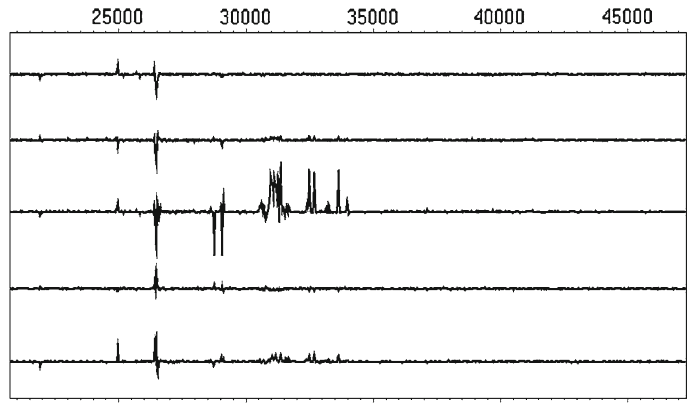
\includegraphics[width=0.65\textwidth]{main thing/Pictures/DPA_diff_trace.png}
    \end{figure}
\end{frame}

\begin{frame}
    \frametitle{Completing the Key Recovery}

    This analysis can be iterated independently for each of the 16 bytes ($n = 0, \ldots, 15$) of the AES state.

    \begin{block}{Important Note}
        The same set of traces can be reused for each round key since each attack tests different hypotheses.
    \end{block}

    This divide-and-conquer approach enables full recovery of the 128-bit AES key.
\end{frame}

\begin{frame}
    \frametitle{Mathematical Formulation of DPA}

    Let:
    \begin{itemize}
        \item $T = \{T_i\}_{i=1}^m$ be the set of collected power traces,
        \item $T_i[j]$ be the power measurement at the $j^\text{th}$ time sample in trace $i$,
        \item $C = \{C_i\}_{i=1}^m$ be the set of known inputs or outputs corresponding to each trace,
        \item $D(C_i, K_n)$ be a binary selection function dependent on known data $C_i$ and a key guess $K_n$.
    \end{itemize}

    Then, the differential trace $\Delta D[j]$ at time offset $j$ for key guess $K_n$ is computed as:

    \[
        \Delta D[j] = 
        \frac{
            \sum_{i=1}^m D(C_i, K_n) \cdot T_i[j]
        }{
            \sum_{i=1}^m D(C_i, K_n)
        }
        -
        \frac{
            \sum_{i=1}^m (1 - D(C_i, K_n)) \cdot T_i[j]
        }{
            \sum_{i=1}^m (1 - D(C_i, K_n))
        }
    \]

    This difference highlights points in time where the power consumption correlates with the selection function’s prediction, helping identify the correct key guess.
\end{frame}


\begin{frame}
    \frametitle{Extending DPA Across Modes and Devices}

    DPA can be adapted for different cipher modes or hardware.

    For example, the figure in the next slide shows a DPA attack on an AES-CBC implementation in an FPGA:

    \begin{itemize}
        \item The ciphertext is available instead of plaintext; so the selection function targets last round key bytes.
        \item A single oscilloscope trace capturing all AES operations is split into many operations for analysis.
    \end{itemize}
\end{frame}

\begin{frame}{Extending DPA Across Modes and Devices}
    \begin{figure}
        \centering
        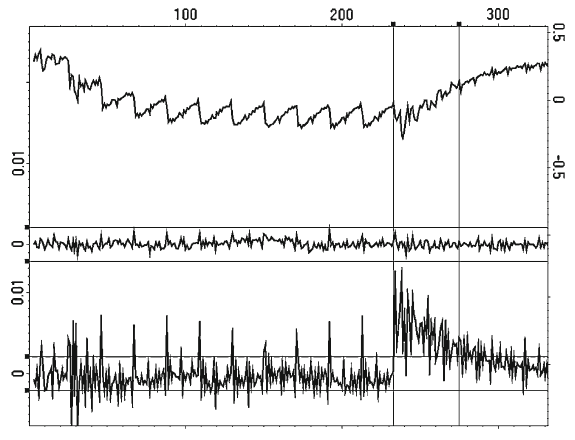
\includegraphics[width=0.75\textwidth]{main thing/Pictures/aes_cbc_fpga.png}
        \caption{DPA results against AES-CBC on FPGA; top: average trace, middle: incorrect key guess, bottom: correct key guess.}
    \end{figure}
\end{frame}










\section{Correlation Power Analysis (CPA)}

\begin{frame}
    \frametitle{From DPA to CPA: Motivation}

    \textbf{CPA} was introduced by Brier, Clavier, and Olivier (2004) as a refinement of Differential Power Analysis. 
    
    \begin{block}{Key Difference from DPA}
        \begin{itemize}
            \item DPA: compares subset averages at a single point in time.
            \item CPA: computes the \textbf{statistical correlation} between predicted leakage
                  (based on a model) and actual power measurements.
        \end{itemize}
    \end{block}
    \vspace{2mm}
    \textbf{Advantage:} Instead of just testing “is there a measurable difference?”, CPA quantifies
    \textit{how well the model matches reality}, across the whole trace.
\end{frame}

\begin{frame}
    \frametitle{Leakage Model 1: The Hamming Weight (HW)}

    The simplest model for data-dependent power leakage assumes consumption is proportional to the number of bits set to '1' in a register or on a bus.

    \begin{block}{Definition: Hamming Weight}
        For an m-bit data word $D = \sum_{j=0}^{m-1} d_j 2^j$, its Hamming Weight is the count of its '1' bits:
        \[
            HW(D) = \sum_{j=0}^{m-1} d_j
        \]
    \end{block}

    \begin{itemize}
        \item \textbf{Key Insight:} In this model, power consumption depends on the \textbf{number of active bits}, not the integer value they represent.
        \item For example, the 8-bit values \texttt{0x01}, \texttt{0x02}, \texttt{0x40}, and \texttt{0x80} all have $HW=1$ and are predicted to leak similar amounts of power.
        \item For uniformly random m-bit data, the average Hamming Weight is $m/2$.
    \end{itemize}
\end{frame}

\begin{frame}
    \frametitle{Leakage Model 2: The Hamming Distance (HD)}
    
    The HW model has a limitation: it ignores the hardware's previous state. A more physically accurate model states that power is consumed when bits \textbf{flip state} (e.g., on a data bus).

    \begin{block}{Definition: Hamming Distance}
        The Hamming Distance between a new data word $D$ and the previous state $R$ is the number of bits that have changed:
        \[
            HD(D, R) = HW(D \oplus R)
        \]
    \end{block}

    \begin{itemize}
        \item This \textbf{transition model} is a better fit for real CMOS logic, where charging and discharging capacitors during bit flips is a major source of dynamic power consumption.
        \item The $D \oplus R$ operation isolates exactly which bits have toggled.
        \item The Hamming Weight model is a special case of the HD model where the reference state $R$ is assumed to be all zeros ($R=0$).
    \end{itemize}
\end{frame}

\begin{frame}
    \frametitle{The Linear Power Model for CPA}

    The Hamming Distance model leads to the fundamental assumption of CPA: the data-dependent portion of the power consumption is linearly related to the number of bit transitions.

    \begin{alertblock}{The Linear Power Model}
    This relationship is expressed as:
    $$ W = a \cdot HD(D,R) + b $$
    \begin{itemize}
        \item $W$: The total power measured at a specific point in time.
        \item $HD(D,R)$: The \textbf{hypothesized leakage} based on the HD model.
        \item $a$: A scaling factor connecting the HD() to the actual power.
        \item $b$: A constant offset representing static power and measurement noise.
    \end{itemize}
    \end{alertblock}
    
    The entire goal of CPA is to find a key guess that makes our hypothesized leakage $HD(D,R)$ strongly correlate with the measured power $W$.
\end{frame}



\begin{frame}
    \frametitle{Limitations of Classic DPA}
    Differential Power Analysis (DPA) distinguishes key guesses 
    by comparing \textbf{average traces across two partitions}.
    
    \begin{itemize}
        \item It only considers the \textbf{difference of means} at each time sample.
        \item It is sensitive to noise: many traces required to average out randomness.
        \item May produce misleading results (\textbf{``ghost peaks''}) when leakage does not align perfectly with the partition.
        \item Wastes information: each sample is treated independently instead of considering correlation across the whole trace.
    \end{itemize}

    \begin{block}{Consequence}
        DPA is useful, but not statistically optimal; it tests for a binary difference instead of measuring \textbf{how strongly traces align with the hypothesis}.
    \end{block}
\end{frame}


\begin{frame}
    \frametitle{Why CPA is a More Powerful Refinement}

    \textbf{Correlation Power Analysis (CPA)} addresses DPA’s shortcomings:

    \begin{itemize}
        \item Uses a \textbf{parametric model} of data-dependent leakage 
              (Hamming Weight or Hamming Distance).
        \item Instead of simply asking \textit{“are two averages different?”}, 
              CPA asks: \newline
            
                  \textit{How well does my predicted power model                 
                  correlate with the measured power trace?}
              
        \item Employs the \textbf{Pearson correlation coefficient} across all traces and all times, 
              giving a continuous score for each hypothesis.
        \item Strong signals stand out as \textbf{statistically significant correlations}, 
              reducing the chance of ghost peaks.
    \end{itemize}

    \begin{block}{Intuition}
        CPA turns DPA from a binary detector into a \textbf{statistical matching process}, 
        making better use of each collected trace.
    \end{block}
\end{frame}

\begin{frame}
    \frametitle{Typical Hardware Setup for CPA}

    CPA requires:

    \begin{itemize}
        \item A device performing cryptographic operations, accessible for power measurement.
        \item A computer that sends known but random data to the device.
        \item A power measurement setup recording traces during device operation.
    \end{itemize}

    \begin{figure}
        \centering
        % Reuse your previous DPA setup image here
        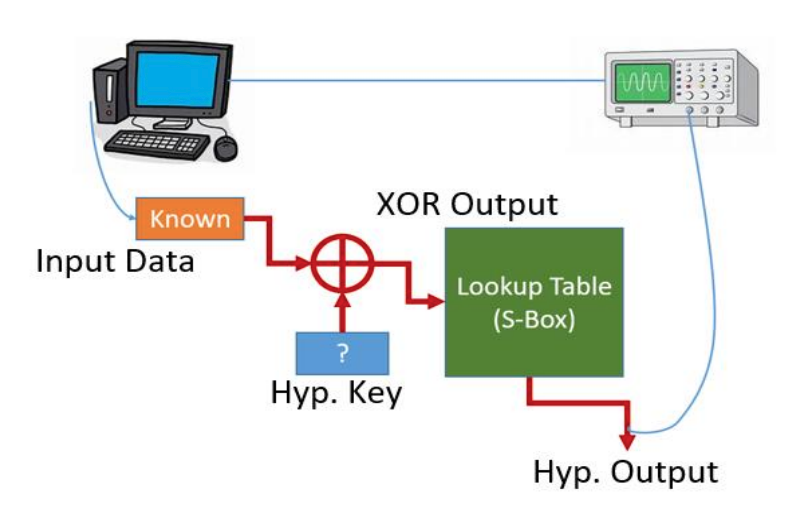
\includegraphics[width=0.7\linewidth]{main thing/Pictures/CPA_setup.png}
        \caption{Typical power measurement setup used in CPA and DPA.}
    \end{figure}
\end{frame}

\begin{frame}
    \frametitle{CPA Attack Strategy}

    The goal of a CPA attack is to find the secret key by identifying which key guess produces a \textbf{predicted power consumption} that best matches the \textbf{measured power consumption}.

    \begin{block}{The Core Question}
        For a given key guess, does the predicted Hamming Weight of an intermediate value (like the S-box output) statistically correlate with the power trace?
    \end{block}

    \begin{itemize}
        \item We perform this process for one key byte at a time.
        \item For AES-128, we target the output of the first round's \texttt{SubBytes} operation, just as we did with DPA.
        \item Intermediate value: $I_{i,n} = S[P_{i,n} \oplus K_n]$.
    \end{itemize}
\end{frame}

\begin{frame}
    \frametitle{CPA Attack on AES}

    The attack iterates through all possible values for a single key byte (e.g., $K_0$). For each guess:

    \begin{enumerate}
        \item \textbf{Hypothesize Intermediate Values:} For each trace $i=1, \dots, N$, calculate the hypothetical S-box output based on the known plaintext $P_i$ and the key guess $K_{guess}$.
        \[ V_{i, guess} = S[P_i \oplus K_{guess}] \]

        \item \textbf{Predict Leakage:} Apply the power model to each hypothetical value. For our example, we use the Hamming Weight model.
        \[ H_{i, guess} = HW(V_{i, guess}) \]
        This gives us a vector of $N$ predicted leakage values for this key guess.

        \item \textbf{Correlate:} Measure the statistical correlation between our vector of predicted leakages ($H_{guess}$) and the vector of actual power measurements at \textbf{each time sample $j$} in the traces.
    \end{enumerate}
\end{frame}

\begin{frame}
    \frametitle{The Tool for the Job: Pearson Correlation Coefficient}

    To quantify how well our predicted leakage matches the real measurements, we use the \textbf{Pearson correlation coefficient} ($\rho$).

    \begin{block}{What it Measures}
        The Pearson coefficient measures the \textbf{strength and direction of a linear relationship} between two sets of data.
    \end{block}

    Its value ranges from -1 to +1:
    \begin{itemize}
        \item $\rho = +1$: Perfect positive linear correlation.
        \item $\rho = -1$: Perfect negative linear correlation (anti-correlation).
        \item $\rho = 0$: No linear correlation.
    \end{itemize}

    \begin{alertblock}{In CPA}
    We compute $\rho$ between our hypothesized Hamming Weights and the measured power trace. A high \textbf{absolute value} of $\rho$ indicates our key guess is likely correct.
    \end{alertblock}
\end{frame}

\begin{frame}
    \frametitle{Pearson Correlation: The Definition}

    The Pearson correlation coefficient ($\rho$) is formally defined as the \textbf{covariance} of two variables, normalized by the product of their \textbf{standard deviations}.

    \begin{block}{Definitional Formula}
    \[
        \rho_{H, T_j} = \frac{\text{cov}(H, T_j)}{\sigma_H \cdot \sigma_{T_j}}
    \]
    \end{block}
    
    \begin{itemize}
        \item $\text{cov}(H, T_j)$: The covariance, which measures how our \textbf{hypothesized leakage vector ($H$)} and the \textbf{measured power vector ($T_j$)} vary together.
        \item $\sigma_H$: The standard deviation of our hypothesized leakage values
        \item $\sigma_{T_j}$: The standard deviation of the power measurements at time sample $j$ 
    \end{itemize}
    Normalizing by the standard deviations removes the units and scale, giving a pure measure of correlation between -1 and +1.
\end{frame}


\begin{frame}
    \frametitle{CPA Results: Identifying the Correct Key}

    After computing the correlation for all 256 key byte guesses at every time sample, we get 256 "correlation traces."

    \begin{itemize}
        \item The plot below shows the correlation traces for a few key candidates.
        \item The trace corresponding to the \textbf{correct key guess} will show a peak
        \item Traces for \textbf{incorrect key guesses} will fluctuate randomly around zero
    \end{itemize}

    \begin{figure}
        \centering
        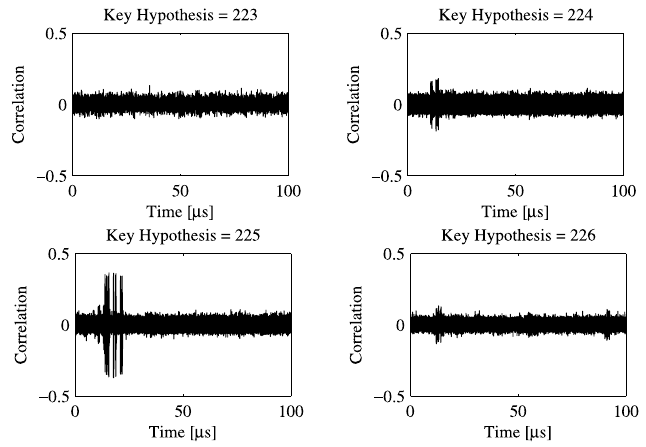
\includegraphics[width=0.7\textwidth]{main thing/Pictures/CPA_correlation_traces.png} 
        
    \end{figure}
\end{frame}

\begin{frame}
    \frametitle{Interpreting the Results: What the Peak Means}

    The peak in the correlation trace for the correct key is the "moment of truth."

    \begin{block}{The Meaning of the Peak}
        \begin{itemize}
            \item The \textbf{X-axis position} of the peak indicates the \textit{point in time} when the target intermediate value (e.g., the S-box output) is being manipulated by the device.
            \item The \textbf{Y-axis value} (the height of the peak) represents the \textit{strength} of the linear correlation ($\rho$). A higher peak means a better model fit and less measurement noise.
        \end{itemize}
    \end{block}
    For the correct key, our hypothesized leakage model, $H = HW(S[P \oplus K_{correct}])$, successfully predicts the device's actual power consumption $W$.
\end{frame}

\begin{frame}
    \frametitle{Interpreting the Results: Incorrect Guesses}
    
    When an incorrect key guess ($K_{wrong}$) is used, the predicted leakage values become meaningless.
    
    \begin{itemize}
        \item The hypothesized leakage vector, $H_{wrong} = HW(S[P \oplus K_{wrong}])$, is now a set of values that are statistically \textbf{independent} of the true intermediate value being processed inside the device.
        \item Therefore, $H_{wrong}$ is also independent of the true data-dependent power consumption, $W$.
    \end{itemize}
    
    \begin{alertblock}{The Result}
        When two data vectors are statistically independent, their Pearson correlation coefficient will naturally approach zero as the number of samples ($N$) increases. This is why the incorrect key traces appear as random noise.
    \end{alertblock}
\end{frame}


\section{Hiding}

\begin{frame}
    \frametitle{Countermeasure Philosophy: Hiding}
    
        Power analysis attacks work because a device's power consumption \textbf{depends on the data} it is processing.
  
    
    \begin{alertblock}{The Goal of Hiding}
        Hiding aims to break the link between the power consumption and the data values. The cryptographic algorithm itself remains unchanged, but its execution becomes difficult to analyze.
    \end{alertblock}
    
    In short, Hiding aims to make the power traces useless to an attacker.
    
\end{frame}

\begin{frame}
    \frametitle{Hiding: Two Fundamental Approaches}
    
    To make power consumption independent of the data, there are two ideal (but theoretical) goals:
    
    \begin{columns}[T]
        \begin{column}{0.5\textwidth}
            \textbf{1. Random Power}
            \begin{itemize}
                \item Make the device consume a \textbf{random} amount of power in each clock cycle.
                \item The real signal is buried in unpredictable noise.
            \end{itemize}
        \end{column}
        
        \begin{column}{0.5\textwidth}
            \textbf{2. Constant Power}
            \begin{itemize}
                \item Make the device consume an \textbf{equal} amount of power in each clock cycle, regardless of the operation or data.
                \item There are no data-dependent variations to exploit.
            \end{itemize}
        \end{column}
    \end{columns}
    
    While perfect randomness or equality is impossible in practice, these two ideals guide all hiding countermeasure design.
    
\end{frame}

\begin{frame}
    \frametitle{Hiding in Practice: Time vs. Amplitude}
    
    Practical hiding techniques can be divided into two groups based on which dimension of the power trace they manipulate.
    
    \begin{block}{1. Manipulating the Time Dimension}
        \begin{itemize}
            \item These techniques randomize \textbf{when} operations occur.
            \item The goal is to misalign the power traces from different executions, making averaging and statistical analysis difficult.
            \item \textit{Example: Random clock jitters or random instruction insertion.}
        \end{itemize}
    \end{block}
    
    \begin{block}{2. Manipulating the Amplitude Dimension}
        \begin{itemize}
            \item These techniques directly alter the power consumption characteristics of the operations themselves.
            \item The goal is to make the power draw for different operations either more random or more uniform.
            \item \textit{Example: Special logic gates that draw constant power.}
        \end{itemize}
    \end{block}
    
\end{frame}

% TIME DIMENSION

\begin{frame}
    \frametitle{Hiding: Time Dimension}

    As we know, DPA and other statistical attacks require \textbf{correctly aligned} power traces to average out noise and isolate the signal.

    \begin{alertblock}{The Countermeasure Strategy}
        If we can randomize the execution of the algorithm, the operations will occur at different moments in time for each run.
    \end{alertblock}

    \begin{itemize}
        \item This misalignment acts as a powerful defense.
        \item An attacker will require significantly more traces to overcome the induced jitter.
        \item The more random the execution, the more difficult the attack becomes.
    \end{itemize}

\end{frame}

\begin{frame}
    \frametitle{Hiding: Time Dimension}

    The basic idea is to randomly insert "do-nothing" or dummy operations before, during, and after the real cryptographic operations.

    \begin{itemize}
        \item In each execution, randomly generated numbers decide how many dummy operations are inserted and where.
        \item The position of each \textit{real} operation now varies randomly from trace to trace.
    \end{itemize}

    \begin{alertblock}{Critical Detail}
        The \textbf{total number} of inserted dummy operations should be constant for all executions. This prevents an attacker from learning anything by simply measuring the total execution time.
    \end{alertblock}

    \begin{block}{Trade-Off}
        More dummy operations provide more security but lead to a \textbf{lower throughput}. A suitable compromise must be found.
    \end{block}

\end{frame}

\begin{frame}
    \frametitle{Time Hiding: Shuffling}

    An alternative to inserting dummies is to randomly change the sequence of operations that can be performed in an arbitrary order.

    \begin{block}{Example: AES S-Box Look-ups}
        \begin{itemize}
            \item In each round of AES, the 16 S-box look-ups are independent of each other.
            \item Their execution order can be \textbf{shuffled}.
            \item In each execution, a randomly generated sequence determines the order of the 16 look-ups, misaligning the leakage for each byte.
        \end{itemize}
    \end{block}

    \begin{columns}[T]
        \begin{column}{0.5\textwidth}
            \textbf{Advantage}
            \begin{itemize}
                \item Does not affect throughput nearly as much as inserting dummy operations.
            \end{itemize}
        \end{column}
        \begin{column}{0.5\textwidth}
            \textbf{Disadvantage}
            \begin{itemize}
                \item Can only be applied to a limited number of independent operations within an algorithm.
            \end{itemize}
        \end{column}
    \end{columns}
\end{frame}

\begin{frame}
    \frametitle{Time Hiding: Software vs. Hardware}

    The effectiveness and options for time-based hiding depend heavily on the implementation level.

    \begin{block}{Software Implementations}
        \begin{itemize}
            \item Dummy operation insertion and shuffling are both easily implemented in software.
            \item However, their protective power is often limited.
            \item A key requirement is a source of good on-device random numbers.
        \end{itemize}
    \end{block}

    \begin{block}{Hardware Implementations}
        \begin{itemize}
            \item Hardware offers significantly more powerful options.
            \item In addition to dummy operations and shuffling, hardware allows for direct manipulation of the clock itself.
        \end{itemize}
    \end{block}

\end{frame}

\begin{frame}
    \frametitle{Hardware Time Hiding: Clock Manipulation}

    In hardware, it is possible to directly randomize the clock signal to destroy trace alignment. Common techniques include:

    \begin{itemize}
        \item \textbf{Random Insertion of Dummy Cycles:} A finer-grained version of dummy operations where individual clock cycles are randomly used for "dummy" computations on random data.

        \item \textbf{Skipping Clock Pulses:} A filter is inserted into the clock path that randomly skips clock pulses, causing jitter.

        \item \textbf{Randomly Changing Clock Frequency:} An internal oscillator's frequency is controlled by random numbers, constantly changing the speed of operations.

        \item \textbf{Multiple Clock Domains:} The device randomly switches between several different on-chip clock signals.
    \end{itemize}

    \begin{alertblock}{}
        For all these techniques, the attacker must not be able to detect the countermeasure (e.g., by observing the clock signal itself).
    \end{alertblock}

\end{frame}

\begin{frame}
    \frametitle{Hiding in the Amplitude Dimension}

    The second major hiding strategy is to directly change the \textbf{power consumption characteristics} of the operations themselves.

    \begin{block}{The Goal: Lower the Signal-to-Noise Ratio (SNR)}
        Recall that the leakage depends on the SNR. The goal is to make this value as close to zero as possible. This can be achieved in two ways:
        \begin{itemize}
            \item Reduce the signal ($Var(P_{op})$) to zero.
            \item Increase the noise ($Var(P_{noise})$) to infinity.
        \end{itemize}
    \end{block}
    
    While the ideal goal of SNR=0 is unreachable, we can get close by either \textbf{increasing the noise} or \textbf{reducing the signal}.

\end{frame}

\begin{frame}
    \frametitle{Amplitude Hiding: Increasing the Noise}

    The goal of this approach is to build a device where random switching activity dominates the power consumption, drowning out the real signal.

    \begin{block}{Hardware Techniques}
        \begin{itemize}
            \item \textbf{Wide Datapaths:} It is harder to attack a single bit in a 128-bit architecture than in a 32-bit one, as more unrelated bits are switching in parallel.
            
            \item \textbf{Noise Engines:} These are dedicated circuits, often based on random number generators connected to large capacitors, whose only job is to create random switching noise in parallel with the real computation.
        \end{itemize}
    \end{block}
    
    \begin{block}{Software Techniques}
        \begin{itemize}
            \item \textbf{Parallel Activity:} Programmers can increase noise by using other components of the device (e.g., coprocessors, communication interfaces) to perform random activities in parallel with the crypto algorithm.
        \end{itemize}
    \end{block}

\end{frame}

\begin{frame}
    \frametitle{Amplitude Hiding: Reducing the Signal}

    The goal of this approach is to make the power consumption as constant as possible, regardless of the operation or data.

    \begin{block}{Hardware Techniques}
        \begin{itemize}
            \item \textbf{Dedicated Logic Styles:} The most common strategy. Cells are built using special logic (e.g., Dual-Rail Pre-charge Logic) designed so that their power consumption is constant, regardless of the input data.
            
            \item \textbf{Power Filtering:} A filter (e.g., using switched capacitors or constant current sources) is inserted between the power supply and the crypto circuit to smooth out data-dependent variations.
        \end{itemize}
    \end{block}
    
    \begin{alertblock}{Important Limitation}
        Hardware-level countermeasures like filtering may not protect against attacks on electromagnetic (EM) emanations, as the EM field is generated before the power is filtered.
    \end{alertblock}

\end{frame}

\begin{frame}
    \frametitle{Amplitude Hiding in Software}

    While software cannot change the power characteristics of the underlying hardware, programmers can make careful choices to reduce leakage.

    \begin{itemize}
        \item \textbf{Choice of Instructions:} Choose instructions that are known to leak less information about their operands.
        
        \item \textbf{Constant Program Flow:} Avoid conditional jumps or branches that depend on the key or secret data. The sequence of executed instructions should always be the same.
        
        \item \textbf{Key-Independent Memory Access:} Avoid memory addresses that depend on the key. If necessary, use addresses that have similar leakage characteristics (e.g., the same Hamming weight).
    \end{itemize}
    
    These software techniques are primarily effective against simpler SPA attacks but are generally not sufficient to defeat DPA.

\end{frame}
\begin{frame}
  \frametitle{Hiding Countermeasures: Summary}
  \scriptsize
  \setlength{\tabcolsep}{4pt}\renewcommand{\arraystretch}{1.2}
  \begin{adjustbox}{\textwidth}
  \begin{tabularx}{\textwidth}{>{\bfseries}l >{\RaggedRight\arraybackslash}X >{\RaggedRight\arraybackslash}X}
    \toprule
     & Time dimension & Amplitude dimension \\
    \midrule
    Goal
      & Randomize when operations occur to misalign traces
      & Lower SNR by equalizing or randomizing power amplitude \\
    Methods
      & Dummy ops; Shuffling; Clock skip; Random freq; Multi-clock
      & Reduce signal (balanced logic, filtering); Increase noise (noise engines, parallel activity) \\
    Notes
      & Throughput overhead; limited shufflable ops; often combined
      & Hardware most effective; software limited; filtering may not help against EM \\
    \bottomrule
  \end{tabularx}
  \end{adjustbox}
\end{frame}



%%%% DRP e WDDL? Vediamo...





\section{Masking} 

\begin{frame}
    \frametitle{Countermeasure Philosophy: Masking}
    
    \textbf{Masking} takes a different approach from Hiding. Instead of changing the device's physical properties, it fundamentally \textbf{changes the data being processed}.
    
    \begin{alertblock}{The Goal of Masking}
        Masking aims to randomize every sensitive intermediate value within the algorithm, making the device's power consumption statistically independent of the true, secret data.
    \end{alertblock}
    
    This is a powerful countermeasure that can provide security even on a "leaky" device.
    
\end{frame}

\begin{frame}
    \frametitle{The Core Idea: Splitting Secrets into Shares}

    Masking is a form of \textbf{secret sharing}. Every sensitive value, $v$, is split into two or more \textbf{shares} that are processed independently.
    
    For a basic first-order scheme, we split $v$ into two shares:
    
    \begin{itemize}
        \item A random value, $m$, called the \textbf{mask}.
        \item The masked value, $v_m$, which is a combination of the secret and the mask.
    \end{itemize}

    \begin{block}{Example: Boolean Masking with XOR}
        The most common method is to use the XOR operation:
        \[ v_m = v \oplus m \]
        The device works with $v_m$ and $m$, but never with $v$ directly. To recover the original value, one simply computes $v = v_m \oplus m$.
    \end{block}
\end{frame}

\begin{frame}
    \frametitle{How Masking Defeats First-Order DPA}

    The security of masking comes from statistical independence.

    \begin{itemize}
        \item The mask, $m$, is a fresh, uniformly random value for each execution.
        \item This means the masked value, $v_m = v \oplus m$, is \textbf{also uniformly random}, regardless of the secret value $v$.
        \item An attacker measuring the power consumption of an operation on $v_m$ will see a value that is statistically independent of $v$.
    \end{itemize}

    \begin{alertblock}{Security Guarantee}
        As long as the attacker can only probe the leakage of a single share at a time (the "\textbf{first-order}" assumption), the leakage they observe contains no information about the secret value. This provides provable security against first-order DPA.
    \end{alertblock}

\end{frame}

\begin{frame}
    \frametitle{A Fully Masked Implementation}

    To be effective, masking must be applied \textbf{throughout the entire algorithm}.
    
    \begin{enumerate}
        \item \textbf{Masking the Inputs:} The plaintext and key are masked at the very beginning of the computation.
        
        \item \textbf{Processing Masked Values:} All subsequent operations in the algorithm must be redesigned to correctly operate on the shares and produce new, correctly masked intermediate results.
        
        \item \textbf{Unmasking the Output:} The final result of the encryption is also masked. The mask must be removed at the very end to produce the correct ciphertext.
    \end{enumerate}
    
    A single unmasked operation at any point can create a fatal vulnerability.
    
\end{frame}

\begin{frame}
    The main difficulty in masking is correctly handling non-linear operations.
    \frametitle{The Challenge of Non-Linear Functions}    
    \begin{block}{Linear Operations are Easy}
        For a linear function $f$ (with respect to XOR), masking is simple because the function distributes over the operation:
        \[ f(v \oplus m) = f(v) \oplus f(m) \]
        The output mask $f(m)$ is easy to compute.
    \end{block}
\end{frame}

\begin{frame}
    \frametitle{The Challenge of Non-Linear Functions}    

    \begin{block}{Non-Linear Operations are Hard}
        For a non-linear function like an AES S-box, this is not true:
        \[ S(v \oplus m) \neq S(v) \oplus S(m) \]
        \begin{itemize}
            \item The relationship between the input mask and the output mask is complex.
            \item Special, and often computationally expensive, "masked S-box" implementations are required to compute the result while keeping all intermediate values properly masked.
        \end{itemize}
    \end{block}

\end{frame}


\begin{frame}
    \frametitle{Types of Masking and Blinding}

    The operation used for sharing defines the type of masking.
    
    \begin{columns}[T]
        \begin{column}{0.5\textwidth}
            \textbf{Boolean Masking}
            \begin{itemize}
                \item Uses XOR ($\oplus$).
                \item $v_m = v \oplus m$
                \item Ideal for bitwise or XOR-based algorithms like AES.
            \end{itemize}
        \end{column}
        \begin{column}{0.5\textwidth}
            \textbf{Arithmetic Masking}
            \begin{itemize}
                \item Uses modular addition or multiplication.
                \item $v_m = v + m \pmod{n}$
                \item Used for algorithms based on arithmetic, like RSA.
            \end{itemize}
        \end{column}
    \end{columns}
    
    \begin{block}{Blinding}
        The term \textbf{blinding} is typically used to refer to arithmetic masking when applied to asymmetric algorithms like RSA.
        \begin{itemize}
            \item \textbf{Message Blinding:} Applying a multiplicative mask to the message.
            \item \textbf{Exponent Blinding:} Applying an additive mask to the private exponent.
        \end{itemize}
    \end{block}
\end{frame}





%implementations of masking



\begin{frame}
    \frametitle{Masking at the Architecture Level: Software}


    \begin{block}{The Basic Software Workflow}
        \begin{enumerate}
            \item XOR the initial plaintext and/or key with a random mask.
            
            \item Ensure all intermediate values remain correctly masked throughout the computation.
            
            \item Keep track of how the mask itself is transformed by the algorithm's operations.
            
            \item Remove the final mask from the output to get the correct ciphertext.
        \end{enumerate}
    \end{block}

    This process is straightforward for linear operations, but non-linear operations (like table look-ups) require special attention.

\end{frame}

\begin{frame}
    \frametitle{The Challenge: Masking Table Look-ups}

    Many modern ciphers, like AES, use table look-ups (e.g., S-boxes) for their non-linear operations. How do you mask a table look-up?

    \begin{block}{The Solution: On-the-Fly Masked Tables}
        Instead of using a fixed table $T(v)$, we must generate a temporary, masked table, $T_m$, for each execution.
        
        \begin{itemize}
            \item The goal is to create a table where looking up a masked input gives a masked output:
            \[ T_m(v \oplus m_{in}) = T(v) \oplus m_{out} \]
            
            \item To build this table, the device must iterate through all possible inputs, calculate the output, and store the correctly masked result in the new table.
        \end{itemize}
    \end{block}
    
    \begin{alertblock}{}
        This process must be repeated for every new mask used. This increases both the \textbf{computational effort} (to build the table) and the \textbf{memory requirement} (to store it), adding significant performance overhead.
    \end{alertblock}
\end{frame}

\begin{frame}
    \frametitle{Random Precharging}

    Random precharging is a simple technique that \textbf{implicitly masks} the power consumption without directly masking the data values themselves.
    
    \begin{block}{How It Works}
        This technique is effective against attacks that exploit the \textbf{Hamming Distance} leakage model (e.g., of a data bus).
        \begin{enumerate}
            \item Before loading a sensitive value, $v$, onto the bus (or into a register), first load a random value, $m$.
            
            \item The device's power consumption will now be related to the Hamming Distance between the random value and the real value: $HD(v, m)$.
            
            \item This is equivalent to leaking the Hamming Weight of the XORed value: $HW(v \oplus m)$.
        \end{enumerate}
    \end{block}
    
    Since the attacker doesn't know the random value $m$, they cannot predict the Hamming Distance.
    
\end{frame}

\begin{frame}
    \frametitle{Pitfall: The Independence Assumption}

    Masking's security proofs often rely on an assumption that can fail in the real world.
    
    \begin{block}{Theoretical Assumption}
        The power consumption of a masked value is independent of the secret.
    \end{block}
    
    \begin{alertblock}{Flaw}
        This assumes leakage depends on only \textbf{one} value at a time. In reality, leakage often depends on the \textbf{relationship between multiple values}, such as the Hamming Distance between consecutive states of a data bus.
    \end{alertblock}
    
    This "combined leakage" can completely break a masking scheme.

\end{frame}

\begin{frame}
    \frametitle{Example: How a Shared Mask Creates a Flaw}
    
    Imagine two values, $v_m$ and $w_m$, that share the \textbf{same mask} ($m$) are processed back-to-back on a device that leaks Hamming Distance.
    \[ v_m = v \oplus m \quad \text{and} \quad w_m = w \oplus m \]
    
    The device's leakage is proportional to:
    \[ HD(v_m, w_m) = HW(v_m \oplus w_m) \]
    
    The math shows the mask cancels out completely:
    \[ HW((v \oplus m) \oplus (w \oplus m)) = HW(v \oplus w) = HD(v, w) \]
    
    \begin{alertblock}{}
        The device leaks information about the \textbf{unmasked} secret values, defeating the countermeasure.
    \end{alertblock}

\end{frame}



\end{document}

%------------------------------------------------------------
%This block of code defines the information to appear in the
%Title page
\title[Power Analysis Side-channel Attacks] %optional
{Side-channel security of superscalar CPUs}

\subtitle{}

\author[Federico Zanca] % (optional)
{Federico Zanca}

\institute[] % (optional)
{
  %\inst{1}%
  Computer Science and Engineering\\
  Politecnico di Milano
  %\and
  %\inst{2}%
  %Faculty of Chemistry\\
  %Very Famous University
}

\date[2025] % (optional)
{}

%\logo{\includegraphics[height=1cm]{overleaf-logo}}

%End of title page configuration block
%------------------------------------------------------------



%------------------------------------------------------------
%The next block of commands puts the table of contents at the 
%beginning of each section and highlights the current section:

\AtBeginSection[]
{
  \begin{frame}
    \frametitle{Table of Contents}
    \tableofcontents[currentsection]
  \end{frame}
}
%------------------------------------------------------------


\begin{document}

%The next statement creates the title page.
\frame{\titlepage}


%---------------------------------------------------------
%This block of code is for the table of contents after
%the title page
\begin{frame}
\frametitle{Table of Contents}
\tableofcontents
\end{frame}
%---------------------------------------------------------







\section{Introduction \& Context}

%---------------------------------------------------------
%Changing visivility of the text
% slide 1
%\begin{frame}
%\frametitle{The Evolving Target: Complex CPUs}
%\begin{block}{Remark}

%\end{block}

%\begin{itemize}
%    \item<1-> Text visible on slide 1
%    \item<2-> Text visible on slide 2
%    \item<3> Text visible on slides 3
%    \item<4-> Text visible on slide 4
%\end{itemize}
%\end{frame}


\begin{frame}
    \frametitle{Recap: What are Side-Channel Attacks?}
    \begin{block}{Definition}
        \begin{itemize}
            \item Side-Channel Attacks (SCAs) exploit unintended physical emanations (e.g., power consumption, electromagnetic radiation, execution time) from a device
            \item These emanations are correlated with the secret data being processed, allowing an attacker to infer sensitive information (e.g., cryptographic keys)
        \end{itemize}
    \end{block}

    \begin{block}{The Fundamental Question }
        \begin{itemize}
            \item How do we accurately \textit{model} these physical emanations to find the leaked information?
            %\item This presentation delves into the specifics of leakage modeling, especially on modern, complex CPUs.
        \end{itemize}
    \end{block}
\end{frame}
%---------------------------------------------------------
%---------------------------------------------------------
\begin{frame}
    \frametitle{Complex CPU Targets}
    \begin{block}{SCA Challenges on Modern CPUs}
    \begin{itemize}
        \item SCAs are increasingly targeting complex platforms:
            \begin{itemize}
                \item SCA targets have evolved from simple micro-controllers and smart-cards to complex single-core and laptop-grade CPUs
                \item Now, side-channel attacks are also relevant for superscalar CPUs
            \end{itemize}
        \item Assessing vulnerability and validating countermeasures becomes significantly more difficult with increasing target complexity
    \end{itemize}
    \end{block}
\end{frame}


\begin{frame}
    \frametitle{Why Microarchitecture Matters for SCA}
    \begin{block}{Main Idea} 
        \begin{itemize}
            \item To assess the side-channel vulnerability of software on a CPU, we \textbf{must} consider the CPU's microarchitectural features.
            \item Correct execution only requires the object code to match the CPU at ISA level.
            \item However, the extent of side-channel leakage also depends on the processor's microarchitecture.
        \end{itemize}
    \end{block}
\end{frame}

\begin{frame}
    \frametitle{Why Microarchitecture Matters for SCA}
    \begin{block}{Dangers of Ignoring Microarchitecture}
        \begin{itemize}
            \item Side-channel countermeasures, if designed without microarchitectural awareness, can be invalidated.
            \item \textbf{Example}: Accidental value combinations due to register reuse, despite careful assembly implementations.
        \end{itemize}
    \end{block}
\end{frame}
%---------------------------------------------------------

%---------------------------------------------------------


\section{Uncovering Microarchitecture via CPI Analysis}






\begin{frame}
    \frametitle{Uncovering Microarchitecture via CPI Analysis}
    \begin{block}{Problem: Hidden Microarchitecture}
        \begin{itemize}
            \item Internal details of CPU microarchitectures (e.g., pipelines, execution units, buffers) are often proprietary and not publicly documented in full detail.
            \item However, precise knowledge of these details is what allows mounting an effective side-channel attack
        \end{itemize}
    \end{block}
\end{frame}

\begin{frame}
    \frametitle{Uncovering Microarchitecture via CPI Analysis}
    \begin{block}{Inferring from CPI}
        \begin{itemize}
            \item A novel method is proposed: using information leaked by the \textbf{Clock cycles Per Instruction (CPI)} achieved on specific instruction sequences.
            \item \textbf{How it works}:
                \begin{itemize}
                    \item Compare CPI of instruction sequences with and without \textit{Read-After-Write (RAW) hazards}.
                    \item Hazard-free sequences reveal best-case CPU capabilities (e.g., dual-issuing).
                    \item Hazard-affected sequences show how hazards prevent parallel execution.
                \end{itemize}
            \item \textbf{Key Interpretations:}
                \begin{itemize}
                    \item A CPI of \textbf{0.5} indicates \textbf{full dual-issuing} (2 instructions per cycle).
                    \item A sustained CPI of \textbf{1} implies a component is \textbf{fully pipelined} (can start a new operation every cycle).
                \end{itemize}
        \end{itemize}
    \end{block}
\end{frame}

\begin{frame}
    \frametitle{Example: ARM Cortex-A7 MPCore}
    \begin{block}{CPU Overview}
        \begin{itemize}
            \item A dual-core, in-order CPU with an 8-stage pipeline.
            \item Described as "partial dual-issue": Not all instruction pairs can be executed simultaneously.
        \end{itemize}
    \end{block}

    \begin{block}{Why Characterize This CPU?}
        \begin{itemize}
            \item Public documentation (reference manuals, GCC backend descriptions) provides a logical view (see next slide).
            \item However, it lacks some microarchitectural details needed for side-channel analysis
        \end{itemize}
    \end{block}
\end{frame}


\begin{frame}
    \frametitle{ARM Cortex-A7 Pipeline Logical View}
    \begin{figure}
        \centering
        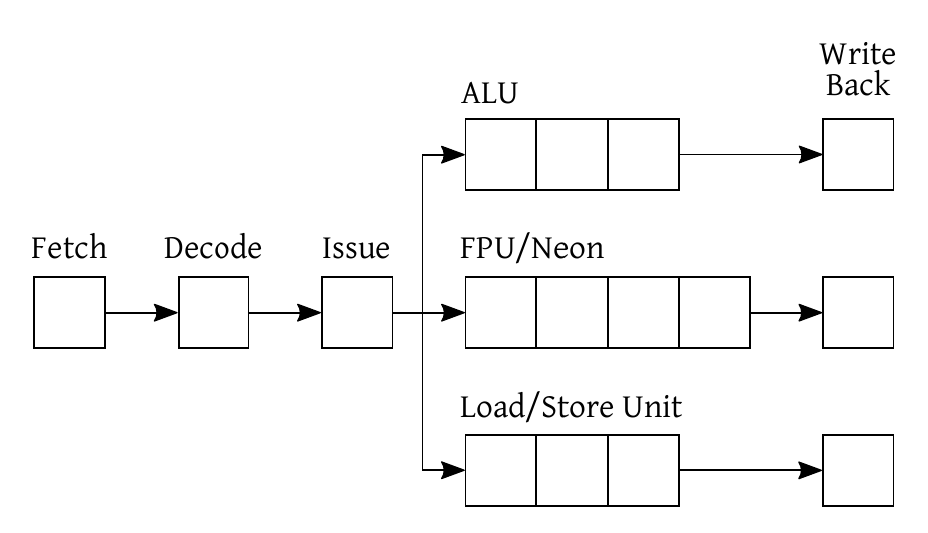
\includegraphics[width=0.8\textwidth]{Pictures/cortexA7.png} 
        \caption{ARM Cortex-A7 MPcore pipeline logical view }
        \label{fig:cortex-a7-pipeline}
    \end{figure}
\end{frame}


\begin{frame}
    \frametitle{Undercovering Microarchitectures (Cortex-A7 Example)}
    \begin{block}{Inferences from CPI Analysis}
        \begin{itemize}
            \item \textbf{ALUs:} Two ALUs are present, but they are not identical. Only one is equipped with a barrel shifter and multiplication unit.
            \item \textbf{Pipelined Units:}
                \begin{itemize}
                    \item The \textbf{Load Store Unit (LSU)} is \textbf{fully pipelined} (sustained CPI of 1 for load/store sequences).
                    \item The \textbf{multiplier} within the ALU is also \textbf{fully pipelined} (CPI of 1 for multiplication sequences).
                \end{itemize}
            \item \textbf{Data Bus Structure:}
                \begin{itemize}
                    \item Three data buses connect the Register File (RF) to the Execution (EX) stage.
                    \item Two buses connect the EX stage back to the RF, implying the RF has two write-ports and three read-ports.
                \end{itemize}
            \item \textbf{Unexpected NOP Behavior:} Counter-intuitively, \texttt{nop} instructions are \textbf{not dual-issued} by the Cortex-A7.
        \end{itemize}
    \end{block}
\end{frame}



\begin{frame}
    \frametitle{Deduction: Cortex-A7 Pipeline Structure}
    \begin{figure}
        \centering
        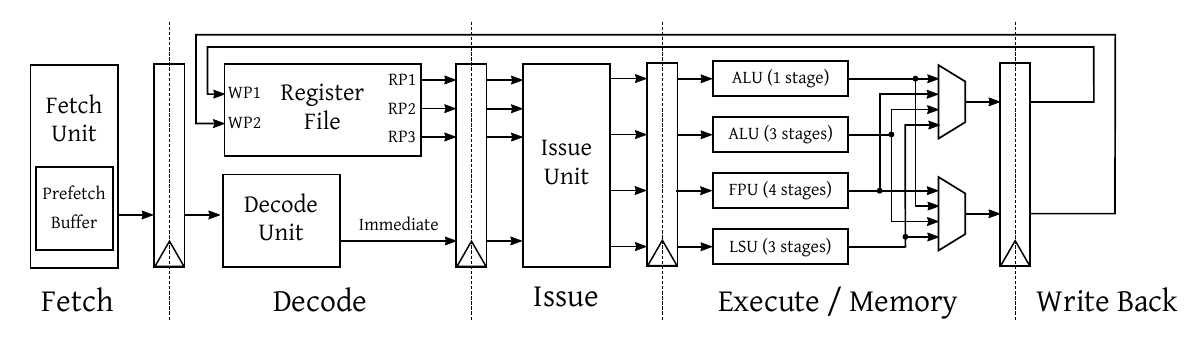
\includegraphics[width=1.0\textwidth]{Pictures/cortexUncovered.png}
        \caption{Alleged ARM Cortex-A7 pipeline structure according to CPI analysis deductions }
        \label{fig:deduced-pipeline}
    \end{figure}
\end{frame}



\begin{frame}
    \frametitle{Dual-Issue Capabilities: Instruction Pairs}
    \begin{table}
        \centering
        \small % makes the content of the table smaller
        \caption{Instruction pairs executed in dual-issue by the Cortex-A7 MPCore CPU. }
        \label{tab:dual-issue-pairs}
        \begin{tabular}{|l|c|c|c|c|c|c|c|}
            \hline
            \textbf{} & \textbf{mov} & \textbf{ALU} & \textbf{ALU w/imm} & \textbf{mul} & \textbf{shifts} & \textbf{branch} & \textbf{ld/st} \\
            \hline
            \textbf{mov}        & \checkmark & \checkmark & \checkmark & \ding{55} & \checkmark & \checkmark & \ding{55} \\
            \textbf{ALU}        & \checkmark & \ding{55}  & \checkmark & \ding{55} & \ding{55}  & \checkmark & \ding{55} \\
            \textbf{ALU w/ imm} & \checkmark & \checkmark & \checkmark & \ding{55} & \checkmark & \checkmark & \checkmark \\
            \textbf{branch}     & \checkmark & \checkmark & \checkmark & \checkmark & \checkmark & \ding{55}  & \checkmark \\
            \textbf{ld/st}      & \checkmark & \ding{55}  & \checkmark & \ding{55} & \ding{55}  & \checkmark & \ding{55} \\
            \textbf{mul}        & \ding{55}  & \ding{55}  & \ding{55}  & \ding{55} & \ding{55}  & \checkmark & \ding{55} \\
            \textbf{shifts}     & \ding{55}  & \ding{55}  & \checkmark & \ding{55} & \ding{55}  & \checkmark & \ding{55} \\
            \hline
        \end{tabular}
    \end{table}
\end{frame}
\section{SCA Characterization \& Leakage Modeling}

\begin{frame}
    \frametitle{Characterizing Microarchitecture Leakage}
    \begin{block}{The Foundation of Leakage}
        \begin{itemize}
            \item Gates driving large capacitive loads are primary sources of side-channel leakage.
            \item Power consumption in such scenarios is well-modeled by the \textbf{Hamming distance} of two values asserted on their outputs in subsequent clock cycles
        \end{itemize}   
    \end{block}

    \begin{block}{Detecting Leakage}
        \begin{itemize}
            \item \textbf{Pearson's correlation coefficient} is used to statistically compare measured power consumption with the predicted leakage model
            \item A correlation statistically distinguishable from zero (with >99.5\% confidence) in the correct clock cycle indicates a leakage
        \end{itemize}
    \end{block}
\end{frame}


\begin{frame}
    \frametitle{Leakage Measurement - Cortex-A7}
    \begin{block}{Data Collection}
        \begin{itemize}
            \item Seven micro-benchmarks: small (2-4) instruction sequences designed to trigger specific component activities
            \item Ran with randomly generated values at each execution, triggered by GPIO
            \item Cache effects eliminated by measuring executions after the first one and inserting 100 \texttt{nop}s
            \item Data acquired: \textbf{100,000 power traces} per benchmark
            \item Each trace was an average of 16 individual executions with the same input, reducing noise
            \item Register File (RF) leakage was evaluated separately by pre-charging destination registers
        \end{itemize}
    \end{block}
\end{frame}

%------------------------------------------------------

\begin{frame}
    \frametitle{Observed Leakage: Registers}
    \begin{block}{Register File (RF)}
        \begin{itemize}
            \item No statistically significant leakage observed from RF read-ports.
            \item Attributed to a short capacitive load, as Issue Stage (IS) buffers drive execution units
        \end{itemize}
    \end{block}
\end{frame}

\begin{frame}
    \frametitle{Observed Leakage: IS/EX}
    \begin{block}{Issue/Execution (IS/EX) Buffers}
        \begin{itemize}
            \item Outputs show significant leakage
            \item \textbf{Modeled by Hamming Distance:} between values of a source operand of an older and a younger single-issued instruction
                \begin{itemize}
                    \item Leakage prominent when operands share the same bus (same source operand position)
                \end{itemize}
            \item \textbf{Hamming Weight Leakage:} Also observed when \texttt{mov}s are interleaved with \texttt{nop}s (due to \texttt{nop} implementation with zero-valued operands)
            \item Dual-issued arithmetic instructions show no measurable leakage among source operands (no shared resources before computation)
        \end{itemize}
    \end{block}
\end{frame}



\begin{frame}
    \frametitle{Observed Leakage: ALUs }
    \begin{block}{ALU and Shift Buffer}
        \begin{itemize}
            \item \textbf{ALU:} Leakage dependent on the \textbf{Hamming weight} of the instruction result
                \begin{itemize}
                    \item Inferred due to ALUs asserting results on previously zero-precharged signals
                \end{itemize}
            \item \textbf{Shift Buffer:} A small leakage proportional to the \textbf{Hamming weight} of the shifted value is present
        \end{itemize}
    \end{block}
\end{frame}

\begin{frame}
    \frametitle{Observed Leakage: EX/WB Buffers}
    \begin{block}{Execution/Write-Back (EX/WB) Buffers}
        \begin{itemize}
            \item Leakage mirrors IS/EX buffers.
            \item \textbf{Modeled by Hamming Distance:} between the \textit{results} of subsequent single-issued instructions.
                \begin{itemize}
                    \item Occurs regardless of destination register sharing or data-flow relationship
                \end{itemize}
            \item \textbf{Hamming Weight Leakage:} Also present for instruction results.
                \begin{itemize}
                    \item Attributed to \texttt{nop} instructions resetting the WB bus to zero 
                \end{itemize}
        \end{itemize}
    \end{block}
\end{frame}




\begin{frame}
    \frametitle{Observed Leakage: MDR}
    \begin{block}{Memory Data Register (MDR) and Align Buffer}
        \begin{itemize}
            \item Potential leakage source during load/store instruction sequences
            \item \textbf{Modeled by Hamming Distance:} between two subsequently loaded or stored values
            %\item Applies even to half-word and single-byte loads/stores (power proportional to HD between full 32-bit words).
            \item Suggests a separate buffer in the Load Store Unit (LSU) for sub-word realignment
            \item Presence of this \textbf{align buffer} and its leakage was confirmed experimentally
        \end{itemize}
    \end{block}
\end{frame}


\begin{frame}
    \frametitle{Superscalar Leakage Modeling}
    \begin{block}{Leakage from Algorithmically Independent Instructions}
        \begin{itemize}
            \item Observed information leakage that combines values from potentially independent instructions, driven by four causes:
                \begin{enumerate}
                    \item Instruction scheduling order
                    \item Position of source operands
                    \item Single or dual-issuing of instructions
                    \item Potential data remanence in LSU buffers
                \end{enumerate}
        \end{itemize}
    \end{block}
\end{frame}
\begin{frame}
    \frametitle{Superscalar Leakage Modeling}
    \begin{block}{Subtle Code Changes can be Harmful}
        \begin{itemize}
            \item Even apparently harmless changes to assembly code (e.g., swapping source operands of a commutative operation like XOR) can lead to side-channel leakage
            \item This is due to altered pipeline resource sharing
            \item Such changes are difficult to detect by tools focusing only on instruction semantics or manual audits
        \end{itemize}
    \end{block}
\end{frame}




\begin{frame}
    \frametitle{Superscalar Leakage: Vulnerabilities}
    \begin{block}{Impact of Dual-Issuing}
        \begin{itemize}
            \item Worsens effects of instruction scheduling and operand position.
            \item Leakage can stem from combinations of source operands of \textit{non-consecutive} instructions if an intermediate instruction is dual-issued
            \item Highlights the crucial, often-neglected importance of instruction scheduling for preventing side-channel leakage
            \item Dual-issuing could also potentially \textbf{enhance security} by enabling parallel computation of two shares in masking schemes
        \end{itemize}
    \end{block}
\end{frame}
\begin{frame}
\frametitle{Superscalar Leakage: Vulnerabilities}
    \begin{block}{Data Remanence and NOPs}
        \begin{itemize}
            \item \textbf{Data Remanence:} In MDR and LSU buffers, old data can accidentally combine with current computation results, creating harmful leakage.
            \item \textbf{NOP Operations:} While semantically neutral, \texttt{nop} instructions can introduce new leakage modes (e.g., by resetting buses to zero). They are not \textit{security neutral}
        \end{itemize}
    \end{block}
\end{frame}





\end{document}